\chapter{Cache Sharing Models}
\label{chap:corun}

In this chapter, we investigate cache sharing models. By applying
footprint into cache sharing models to predict and evaluate program
co-locating penalties, we propose two cache sharing models, iterative
model and pressure-sensitivity model. While iterative model provides
in-depth insight on circular effect of program corun interference,
pressure-sensitivity model gives a simple 2-step solution on
interference prediction. Both models are offline cache sharing models
and are evaluated to be accurate in performance prediction. 

\section{Iterative Cache Sharing Models}
\label{sec:iter-model}
A basic question in multi-core processor design is whether to use
partitioned or shared cache.  Partitioned cache can be wasteful when
only one program is running.  Shared cache is risky since programs
interfere with each other. To answer this question, cache sharing
models are essentially important. Accurate cache interference
predictions are the key to improve the throughput and ensure the
fairness for a set of co-running programs. 

Recall the introduction of cache sharing models in
Chapter~\ref{chap:intro}, cache sharing models can be loosely divided
into on-line and off-line types.  On-line models are used to minimize
the interference among programs that are currently being executed on a
given machine.  Off-line models do not improve performance directly
but can be used to understand the causes of interference and to
predict its effect before running the programs (so they may be grouped
to reduce interference). Compared to on-line models which usually only
consider cache misses, off-line analysis takes all data accesses into
account and provides clean-room statistics that make the cache sharing
models composable. Composition is superior to exhaustive testing,
especially when the corun options are exponential to the number of
tasks. In this chapter, we will mainly focus on offline cache sharing
models. 

\subsection{Off-line Analysis}
Before we explore the iterative models, let us briefly review some
basic concepts in offline cache sharing models.   
For each memory access, the temporal locality is determined by its
reuse window, which includes all data access between this and the
previous access to the same datum.   Specifically, whether the access
is a cache (capacity) miss depends on the reuse distance, the number
of distinct data elements accessed in the reuse window. 
The capacity miss rate can be defined by a probability function
involving the reuse distance and the cache size.  Let the test program
be $A$. 

\begin{equation*}
\begin{array}{l}
  P(\mbox{capacity miss by A alone}) = P(\mbox{A's reuse distance $\ge$ cache size})
\end{array}
\end{equation*}

Let $A,B$ be two programs share the same cache but do not shared
data. Reuse windows in program $A$ concur with time windows in program
$B$.  The reuse distance of $A$ is lengthened by the footprint of
$B$'s window. The effect of $B$ on the locality of $A$ is shown in the
following equation, where $rd$ and $fp$ are short for reuse distance
and footprint correspondingly.  

\begin{equation*}
\begin{array}{l}
 P(\mbox{capacity miss by A(with B)}) = P(\mbox{(A's rd + B's fp) $\ge$ cache size})
\end{array}
\end{equation*}

An implication of the cache sharing model is that cache interference
is asymmetric if locality and footprint are different metrics of a
program.  A program with large footprints and short reuse distances may
disproportionally slowdown other programs while experiencing little to
no slow down itself.  This is confirmed in our experiments.  In one
program pair, the first program shows near 85\% slowdown while the
other program shows only 15\% slowdown.

\subsection{Iterative Models}

Shared cache is a dynamic system.  The interaction between active
programs is likely non-linear since the cause and effect form a loop.
The memory access of one program affects the performance of its peers,
whose effect ``feed back'' to itself.  In this section we first
express this relation in an equation system and then present our
solution.

Let programs 1 and 2 of infinite length run on shared cache. Their
speeds, measured by cycles per instruction, are denoted as $cpi_1,
cpi_2$ correspondingly when running alone. When they execute together,
their speed may change. We use $\delta_1, \delta_2$ to denote the
speed changes for program 1 and 2 correspondingly. If we assume
uniform speed change, an original time window of size $t$ in an
individual execution will take time $t\delta_1$ in program 1 and
$t\delta_2$ in program 2. We call this effect \emph{execution
  dilation} and the term $\delta_i$ the dilation factor of program
$i$. 

With execution dilation, we can easily compute that a reuse window
of size $t$ in program 1 concurs with a footprint window of size
$t\frac{cpi_1\delta_1}{cpi_2\delta_2}$ in program 2. The equation of
capacity misses in shared cache is extended to

\begin{equation}
\label{eq:x}
P(\mbox{capacity miss by P1(with P2)}) = P\left[d_1 + f_2\left(t(d_1)\frac{cpi_1\delta_1}{cpi_2\delta_2}\right) \ge C\right]
\end{equation}

\noindent where $d_1$ is a reuse distance of program 1, $t(d_1)$ is the
size of reuse window of $d_1$ when program 1 is running alone, $f_2(x)$ is
the footprint of program 2 in a window of size $x$, and $c$ is the
size of shared cache. The relative increase in shared-cache misses
for program 1 is computed as $x_1$ as below. The relative increase in
shared-cache misses for program 2 is similarly computed as $x_2$.

\begin{equation}
\label{eq:x}
x_1 = \frac{P\left[d_1 + f_2\left(t(d_1)\frac{cpi_1\delta_1}{cpi_2\delta_2}\right) \ge C\right]}{P\left[d_1 \ge C\right]}
\end{equation}

To connect caching effect with execution time, we need a timing model.
An accurate model is highly unlikely to exist given the complexity of
modern computers.  For example, the penalty of a cache miss on an
out-of-order issue processor depends on the parallelism with
surrounding instructions, the overlapping with other memory accesses,
and the choice of hardware or software prefetching.  Instead of
looking for an accurate model, we use a simple model that can capture
some first-order effect in the relation between cache misses and
execution time.  

We use a linear model, $T = T^n n + T^p m^p + T^s m^s$, where $T$ is
the execution time, $n$ is the number of instructions, $m^p$ is the number
of private-cache misses, $m^s$ is the number of shared-cache misses,
and $T^n, T^p, T^s$ are the average cost of an instruction, a
private-cache miss, and a shared-cache miss.  Of the 6 factors, $n,
m^p, m^s$ are trace specific, and $T^n, T^p, T^s$ are machine
specific.  The values of $T^n$, $T^p$, and $T^s$ are learned by 
linear regression given the linear model and a set of measured
execution times  and predicted L1 and L2 cache misses from SPEC2K
benchmarks. The product of $T^n n$ can be viewed as the execution time
when all data access are cache hits.  The other two factors, $T^p m^p,
T^s m^s$, are the penalty from cache misses.  We make the simplifying
assumption that all misses have the same penalty.  A similar
assumption was used by Marin and
Mellor-Crummey~\cite{MarinM:SIGMETRICS04}. 

% MarinM:LACSI05

Combining the cache model and the time model, the dilation factor for
program $i$($i=1,2$) can be derived by the following equation. 

\begin{equation}
\label{eq:delta_i}
\frac{T^n n_i + T^p m^p_i + T^s m^s_i x_i}{T^n n_i + T^p m^p_i + T^s m^s_i} = \delta_i
\end{equation}

\noindent Substituting $x_i$ with its equation, we have two recursive
equations of two unknowns, $\delta_i$.  The formulation can be
extended to $p$ programs by changing the equation for $x_i$ to the
following equation and generating $p$ equations with $p$ unknowns.  

\begin{equation}
\label{eq:x_i}
x_i = \frac{P\left[d_i + \Sigma_{j\ne i}f_j\left(t(d_i)\frac{cpi_i\delta_i}{cpi_j\delta_j}\right) \ge C\right]}{P\left[d_i \ge C\right]}
\end{equation}

The recursive equations are solved using an iterative method.  We first
set $\delta_i$ to be 1, use the equations to compute the new value of
$\delta'_i$, and repeat until all $\delta_i$ stops changing
($|\delta'_i-\delta_i| < \epsilon \delta_i$, where $\epsilon$ is set
to 0.01 in our experiments).

To analyze the convergence property of the solution, consider the
2-program run case.  We symbolize $x_i$ in Equation~\ref{eq:x_i} as a
function $x_i(\frac{\delta_1}{\delta_2})$.  Substituting this function
into Equation~\ref{eq:delta_i} for $\delta_1,\delta_2$ and putting one
over the other we have

\begin{equation}
\label{eq:fp}
\frac{\frac{T^n n_1 + T^p m^p_1 + T^s m^s_1 x_1\left(\frac{\delta_1}{\delta_2}\right)}{T^n n_1 + T^p m^p_1 + T^s m^s_1} }
{\frac{T^n n_2 + T^p m^p_2 + T^s m^s_2 x_2\left(\frac{\delta_1}{\delta_2}\right)}{T^n n_2 + T^p m^p_2 + T^s m^s_2} }  = \frac{\delta_1}{\delta_2}
\end{equation}

\noindent If we represent the left-hand size as a function $F$, the
equation becomes $F(\frac{\delta_1}{\delta_2}) =
\frac{\delta_1}{\delta_2}$.  Following theorem ensures the convergence of our 
iteration model.

\begin{theorem} 
$\exists \delta_1,\delta_2$, such that $\frac{\delta_1}{\delta_2}= F(\frac{\delta_1}{\delta_2})$.
\end {theorem}
\begin{proof}
Let $r=\frac{\delta_1}{\delta_2}$. 
According to the definition of $F$, we have the following 3 statements immediately. 
\begin{itemize}
\item $y=F(r)$ is non-decreasing. Notice, when $r$ increases $x_1(r)$ increases while $x_2(r)$ decreases. 
\item $F(0_+)=C1>0$, where C1 is constant.
\item $F(\inf)=C2<\inf$, where C2 is constant.
\end{itemize}
Let $r_1=max$ $S_1$, where $S1=\{r|\forall s \le r, F(s) \ge s\}$,  
$r_2=min$ $S_2$, where $S2=\{r|\forall s<r, F(s) \ge s, F(r) \le r\}$. 
Obviously $r_1 \le r_2$. we claim $r_1=r_2$.
\indent

Assume $r_1 \ne r_2$ by contradiction.
According to the definition of $r_1$, $F(r_1) \ge r_1$,
which means $F(r_1) \not\in S_1$.
According to the definition of $r_2$, $F(r_1) \in S_2$, which means 
$F(r_1) \ge r_2$.  Because $F(r_2) \le r_2$, we have $F(r_1) \ge F(r_2)$, 
which contradicts the assumption that $F(r)$ is non-decreasing.
Since $r_1=r_2$ by definition, we conclude $F(r_1)=r_1$.
\qed
\end{proof}

This iterative cache sharing model can be easily scale to $n$ programs
situation. To run $n$ programs on a machine with $p$ processors, there
are $n \choose p$ choices of co-execution. Our model can capture the
asymmetrical and iterative effect of cache sharing by accurately
predict each program's execution dilation. Users can rank the corun
choices according to the dilation and choose program combinations
that have least interference. 

\section{Pressure and Sensitivity Models}

The idea of pressure-sensitivity model is to use two intuitive
metrics, cache pressure and cache sensitivity, to characterize the
programs in a shared cache environment. Pressure is the effect a
program imposes on the system and in turn on its peer
programs. Sensitivity is how strong the program responds to the
pressure imposed by the system or peer programs. While low
pressure means more ``friendly'' or ``polite'' to other programs, low
sensitivity indicates high defensiveness against unknown peers. We
call the new metrics together as the program's personality.  

There are different ways of computing cache pressure and
sensitivity. For example, Bubble-Up system proposed by Mars et
al.~\cite{Mars+:IEEEM12} devised special utilities, reporter and
bubble-up, to test pressure and sensitivity correspondingly. However,
their measurement is machine dependent and corun testing dependent. 

We use program intrinsic metrics to derive pressure and
sensitivity. The key concept used here is the fill time(short for
volume fill time in Section~\ref{subsec:lf}), which can be
derived from average footprint. To help with the presentation, we show
the high-level relations among different concepts as well as the input
and the output of information in Figure~\ref{fig:roadmap}.

\begin{figure}[h!]
\centering
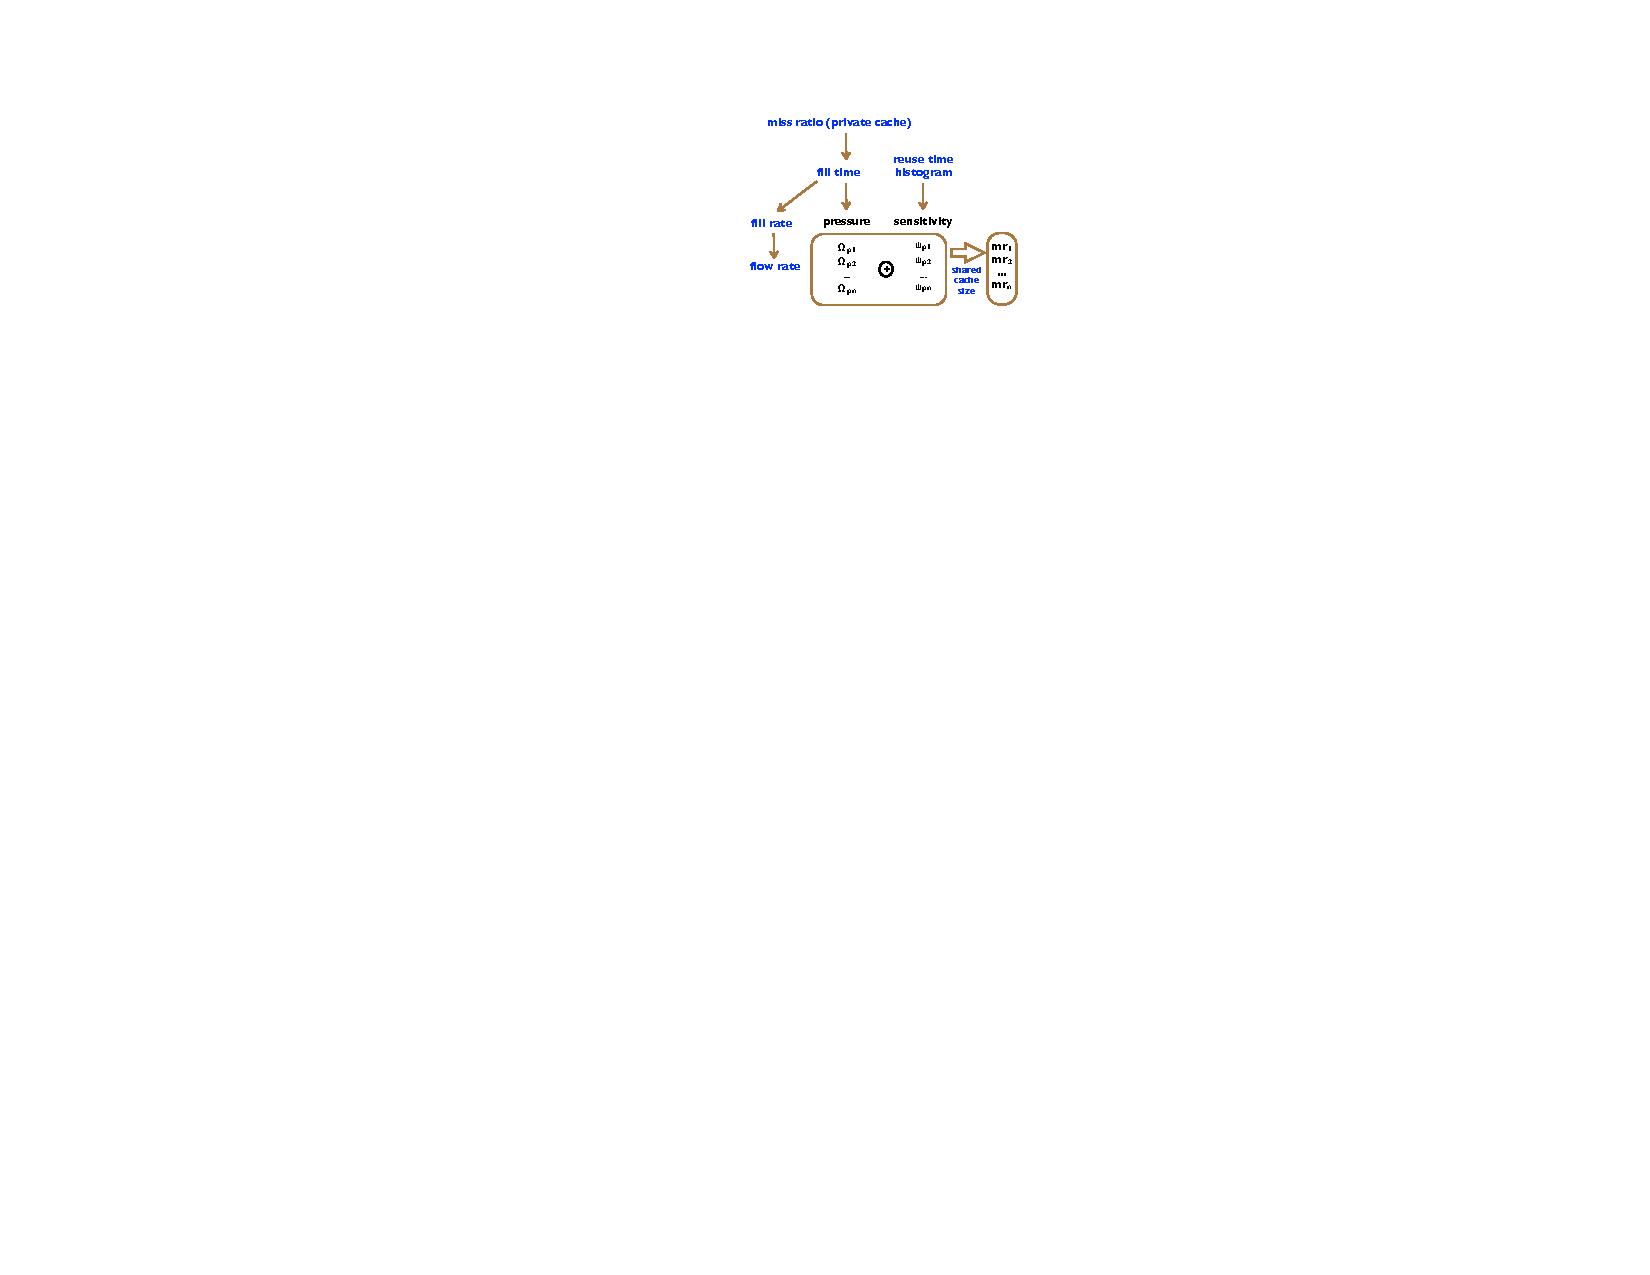
\includegraphics[width=0.7\textwidth,type=pdf,ext=.pdf,read=.pdf]{figures/corun/feeling_roadmap} 
\caption{Cache pressure and sensitivity are computed from the miss ratio and reuse time histogram in private cache and used to compute the miss ratios in shared cache}
\label{fig:roadmap}
\end{figure}

\subsection{Fill Time, Fill Rate, and Flow Rate}
\label{sec:fill_time}

Recall the concept introduced in Section~\ref{subsec:lf}. The volume fill
time is the time a program takes to access a given amount of data, or
symbolically, $vt(v)$ for volume $v$. We define the cache fill time as
the time a program takes to access the amount of data equal to the
size of the cache, or symbolically $vt(c)$, where $c$ is the cache
size.  It is important here we count all accesses in this definition.
An alternative is to count only cache misses --- the time a program
takes to load through cache misses the same amount of data as the
cache size.  To distinguish the two, we call the former the
\emph{access fill time} and the latter the \emph{miss fill time}.  The
two are equivalent if the cache is empty.  But in the ``warm'' cache,
the miss fill time is the upper bound of the access fill time.  The
relation is intuitive if we consider that by counting only misses, we
ignore the effect of cache hits and hence we under-estimate the cache
activity and over-estimate the fill time. If not mentioned
explicitly, by fill time we always mean access fill time.

We have already shown in Section~\ref{subsec:lf} how to precisely compute
the volume fill time. The invariant $fp(vt(c)) = fp(fp^{\ -1}(c))= c$
symbolizes the conversion that when the footprint is the cache size,
the footprint window is the fill time. The conversion is shown
visually in Figure~\ref{fig:fp2vt}.  From the average footprint curve,
we find the cache size $c$ on the y-axis and draw a level line to the
right.  At the point the line meets the curve, the $x$-axis value is
the fill time $vt(c)$. The function of computing the fill time is the
inverse function of computing the average footprint.

\paragraph{The Fill Rate}
If we inverse of the fill time, we get the \emph{fill rate} $fr(c)$.  

$$fr(c) = \frac{1}{vt(c)}$$

\noindent It shows the percentage of cache a program fills at a unit
time.  For example, if a program takes 4 seconds to fill the 4MB
cache, the fill rate is 1/4 = 25\%.  Each second, the program fills
25\% of the cache.  The fill rate makes it convenient to compare the activities by co-running programs.  A program with a higher
fill rate produces greater interference.  

\paragraph{The Flow Rate}
While the fill rate measures the activity in cache by a relative size,
the flow rate measures it directly by the data volume:

$$fr'(c) = fr(c) * c$$

\noindent If the fill rate is 25\% a second for the 4MB cache, the
flow rate is 1MB per second.  

\bigskip 

From the formulas, a program may exist for which the fill rate
decreases with the cache size while the flow rate increases.  However,
our new theory of locality in Chapter~\ref{chap:model} shows that the
average footprint (the average amount of data accessed in a time
interval) is a non-decreasing concave function over the length of the
time interval.  We omit the derivation here, but we can prove as a
corollary that the flow rate is non-increasing with the cache size.
From the same theorem, we can prove that the fill rate is
non-increasing and convex as a function over the cache size. 

The fill rate and the flow rate are composable in that the combined
rate of a set of programs is the sum of their individual rates.
However, the resulting rate cannot be used directly to compute the
miss ratio in shared cache.  For this purpose, we next present the
pressure function.

% explain this a bit?

\subsection{The Cache Pressure}

The pressure is the inverse of the fill time.  As a function, the fill
time maps the cache size to time.  The pressure function, which we
denote as $\Omega( ft )$, the size of the cache that is filled in time
$ft$.  Since the cache pressure and the fill time are inverse
functions of each other, we have the following equality:

$$\Omega( ft( c ) ) = c$$

\noindent The invariance symbolizes the relation that when the time is
the fill time, the pressure is the cache size. Since we have already
proved that average footprint is the inverse function of the fill
time, the pressure curve is the average footprint curve with a different
$x$-axis.  Instead of showing the average footprints over different
window lengths(logical time), it shows the average footprints over
varying time window(real time). 

Figure~\ref{fig:bzip2_pressure} shows the cache pressure of
\emph{bzip2}, a program from the SPEC 2006 benchmark suite running on
one of the reference inputs.  Between 0 and 0.006 second, it fills the
cache up to 2.5MB in size.  To compute this pressure function, we first
compute the average footprint function and then translated the logical
time, i.e. number of memory accesses, to real time based on the
measured run time, by multiplying the inverse of data access rate.

\begin{figure}[h!]
\centering
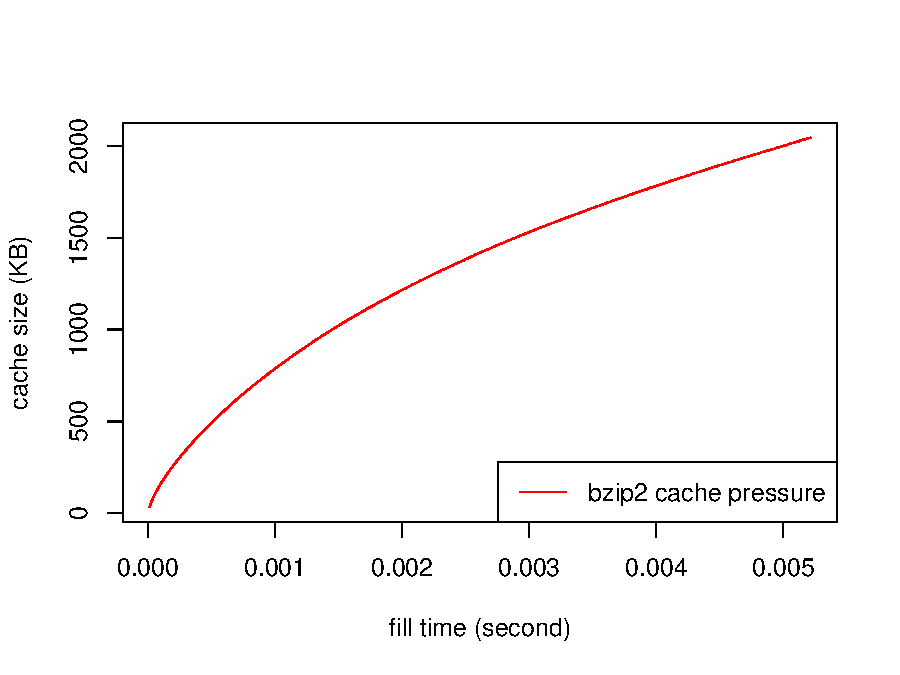
\includegraphics[width=0.7\textwidth,type=pdf,ext=.pdf,read=.pdf]{figures/corun/bzip2_pres} 
\caption{The cache pressure of \emph{bzip2} from SPEC 2006}
\label{fig:bzip2_pressure}
\end{figure}

The cache pressure of \emph{bzip2} is curved, as the figure shows.
Initially, it accesses new data at a rapid rate.  As more data are in
cache, the rate of new data access decreases, indicating an increase
in data reuse, i.e. locality.  Note that we can see the effect
of locality because our definition of the fill rate considers all data
accesses.  If we consider just cache misses, the pressure function
would be strictly linear, as shown in Figure~\ref{fig:miss-fp-comp}.
In fact, this is the reason that the fill rate from multiple programs
can be added but the miss ratios cannot be. 

The use of the pressure function will be clear after we define the
sensitivity function and when we show how the two are used together.

\subsection{The Cache Sensitivity}

Cache sensitivity is how much a program's miss ratio changes with the
cache pressure.  The pressure, as defined earlier, is the fill time.
The higher the pressure is, the shorter the fill time will be.  The
sensitivity shows how quickly the miss ratio increases as the fill time
decreases.

There is a simple relation between the fill time and the miss ratio.
The relation depends on the reuse time, that is, how long the access
happens after the previous access to the same datum.  After the
previous access, if the cache has enough time to be filled, the cached
copy will have been evicted by the time of the reuse, so the access
will be a miss.  For fully associative LRU cache, the condition is
necessary and sufficient.  A data access is a miss if and only if the
reuse time is greater than the cache fill time.

The sensitivity function is one minus the cumulative distribution of
the reuse times.  When the fill time is zero, the cumulative
distribution is 0, and the miss ratio is 100\%.
Figure~\ref{fig:bzip2_sens}(a) shows the reuse time histogram of
\emph{bzip2}, and computed from it, the cache sensitivity in
Figure~\ref{fig:bzip2_sens}(b).  The three peaks in the histogram show the
concentration of reuse times between 0.0015 and 0.03 second.  If due to
cache pressure that the fill time drops below 0.0015 second, the reuses
in the three peaks will become misses, increasing the miss ratio
sharply.  On the other hand, these reuses will always be cache hits,
insensitive to the change in cache pressure if the fill time stays
over 0.03 second.  The range of pressure in which
\emph{bzip2} is sensitive is between 0.0015 and 0.03 second in fill time.

\begin{figure}[h!]
\centering
  \subfigure[the reuse time histogram]{
    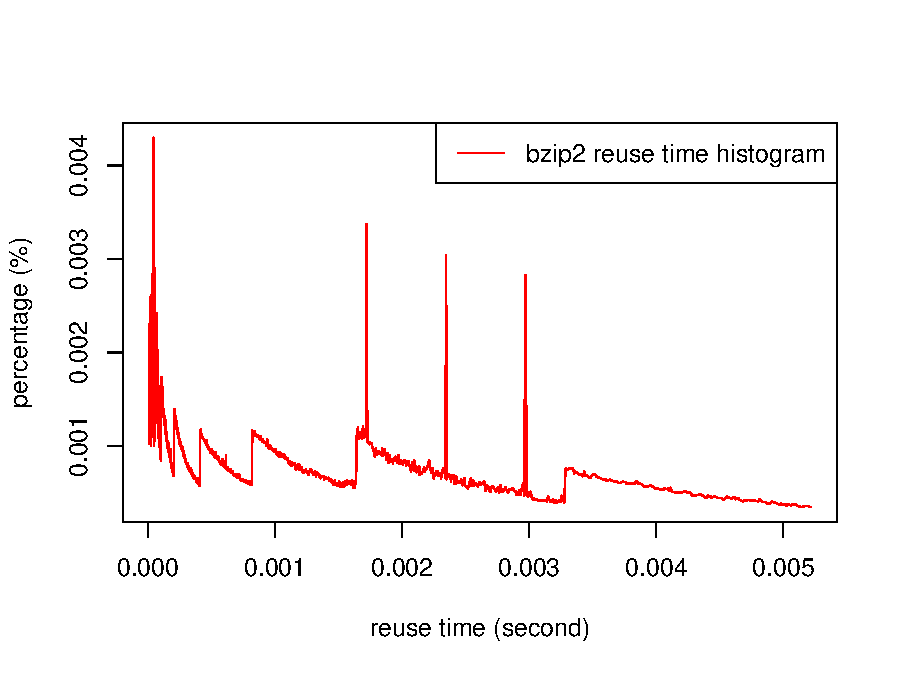
\includegraphics[width=7.5cm,type=pdf,ext=.pdf,read=.pdf]{figures/corun/401.bzip2.time_rt}
  }%\hfill
  \subfigure[the cache sensitivity]{
    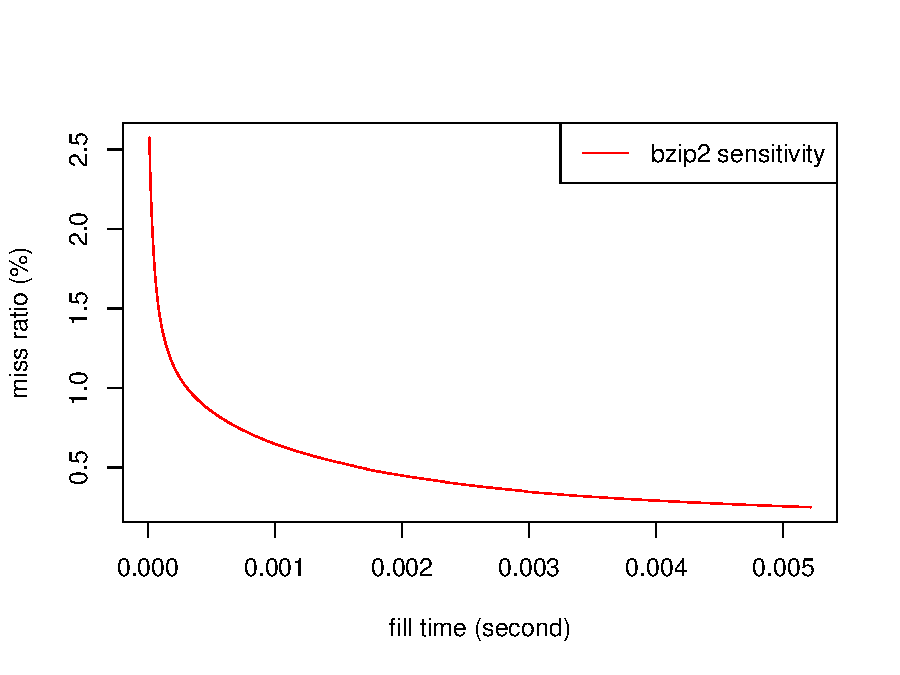
\includegraphics[width=7.5cm,type=pdf,ext=.pdf,read=.pdf]{figures/corun/bzip2_sens}
 }\hfill
\caption{The reuse time histogram (a) is used to compute the cache sensitivity (b) in \emph{bzip2}}
\label{fig:bzip2_sens}
\end{figure}

The sensitivity curve is the miss-ratio curve with a different
$x$-axis.  Instead of showing the miss ratios over different cache
sizes, it shows the miss ratios over varying cache pressure.  Next 
we connect the pressure and the sensitivity metrics together.

\subsection{Solo-run Miss Ratio Prediction}

As an intermediate step, we first show the composition of the pressure
and sensitivity to predict the miss ratio of a single program running
by itself.  Its pressure plot maps from the cache size to the fill
time.  The sensitivity plot gives the miss ratio for that fill time.
Figure~\ref{fig:bzip2_compute_mr} shows these two steps for the
example program \emph{bzip2}.  The three arrow lines show the direct
conversion from the cache size to the fill time and then to the miss
ratio.  Only the pressure and the sensitivity plots are needed in the
conversion.  

\begin{figure}[h!]
\centering
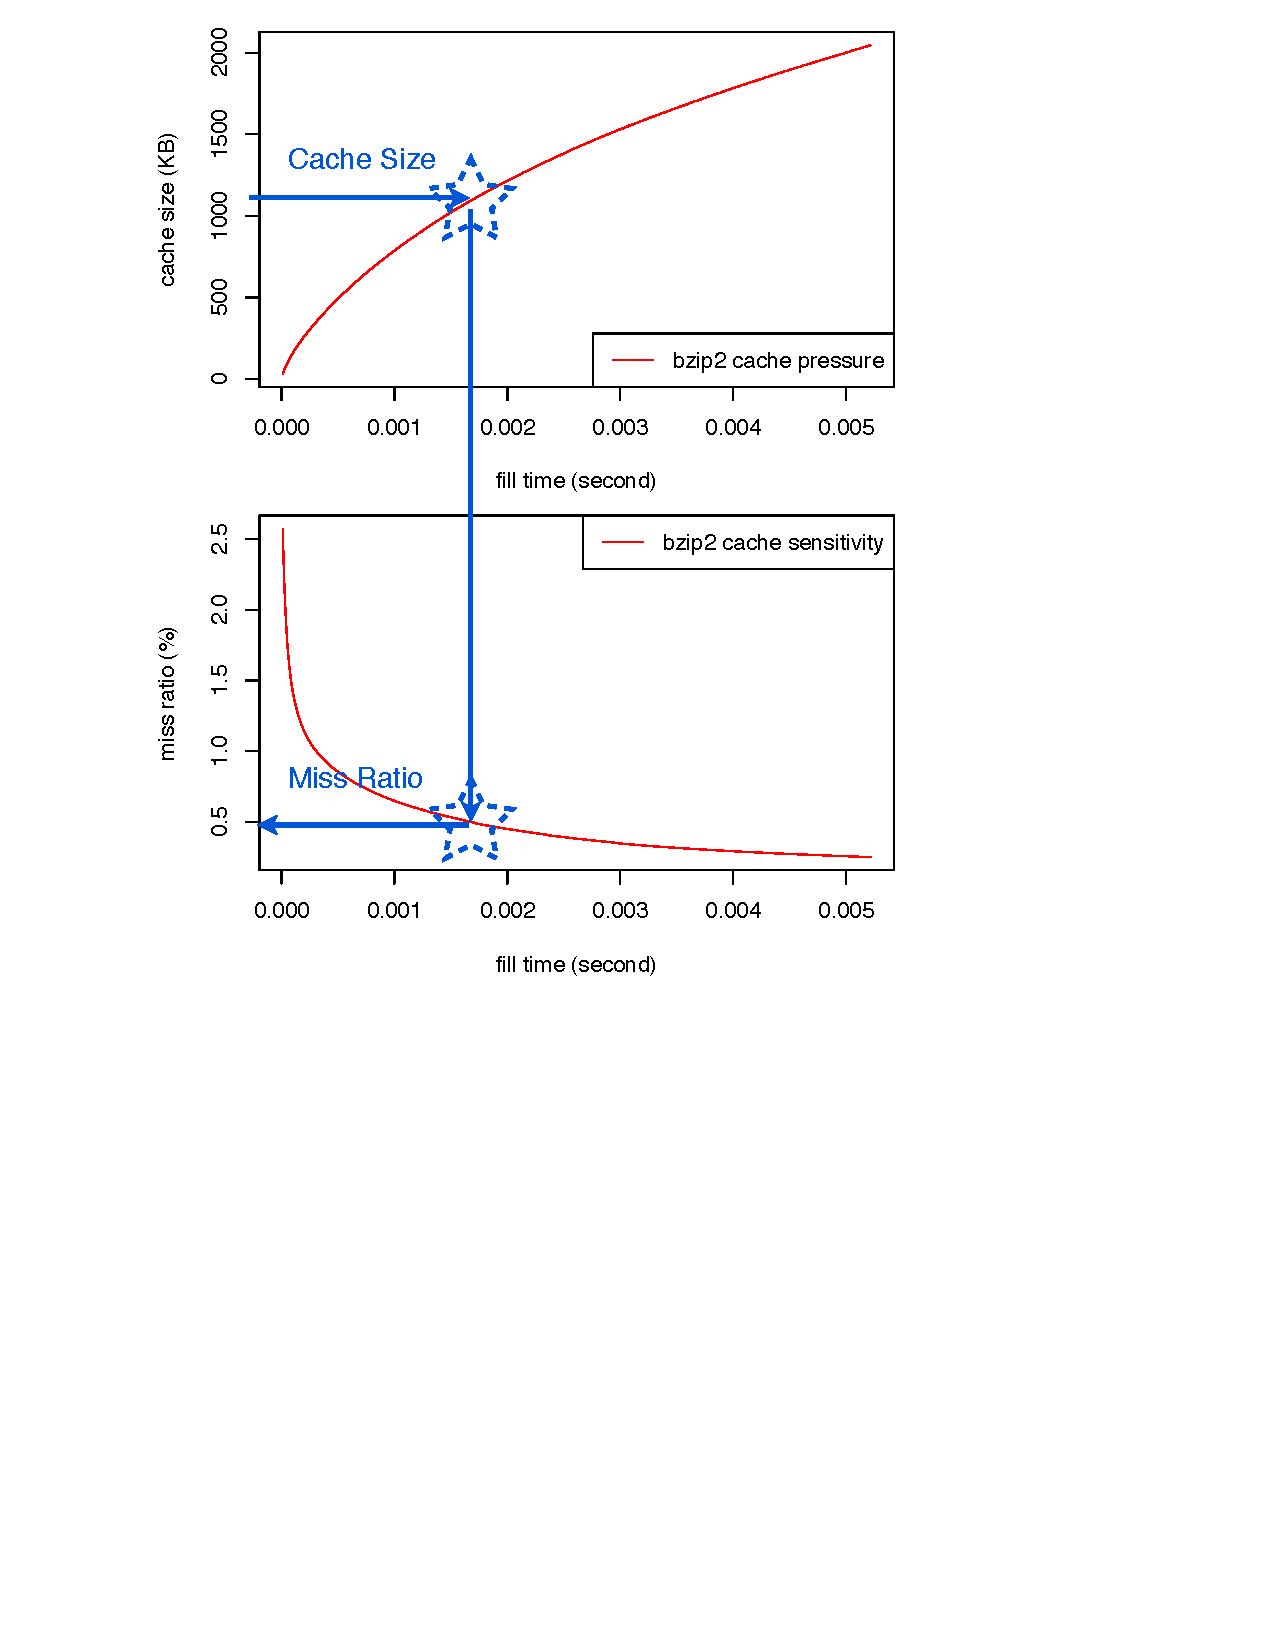
\includegraphics[width=7.5cm,type=pdf,ext=.pdf,read=.pdf]{figures/corun/bzip2_compute_mr}
\caption{The solo execution of \emph{bzip2}.  The miss ratio $M$ is predicted for cache size $C$ using the cache pressure and sensitivity. }
\label{fig:bzip2_compute_mr}
\end{figure}

As a test, we predict the solo-run miss ratios for a machine with 4MB
last level cache and compare it with the measurement from the hardware
counters.  The exact setup will be described in the evaluation
section.  Here we show a quick comparison in
Figure~\ref{fig:seq_mr_comp} to convince the reader that these
abstract concepts can be useful in modeling what actually happens in
the cache of a real machine.  The most interesting evaluation will be
given in the evaluation section for the cache sharing prediction.

\begin{figure}[h!]
\centering
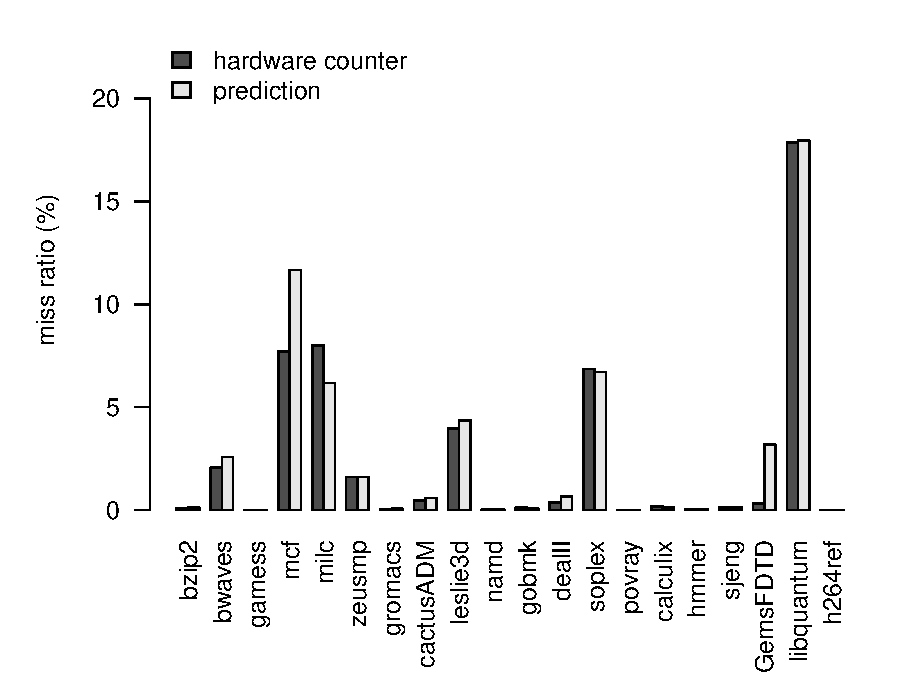
\includegraphics[width=0.7\textwidth,type=pdf,ext=.pdf,read=.pdf]{figures/corun/seq_mr_comp}
\caption{The solo-run miss ratio prediction of SPEC2006 benchmarks
  compared with the hardware counter results}
\label{fig:seq_mr_comp}
\end{figure}

The pressure-sensitivity composition can predict the miss ratio for
any cache size.  Effectively, the result is the miss ratio curve.  
The modeling of pressure and sensitivity is a balance between
simplicity and accuracy.  In design, the models are simple to compute
and use.  Whether they are useful in practice completely depends on
their accuracy, which we will evaluate empirically, after we show the
main purpose of the models in the next section.

\subsection{Co-run Miss Ratio Prediction}

The co-run prediction generalizes the two steps of the solo-run
prediction as follows.  In the first step, the pressure of all co-run
programs is added to produce the combined pressure.  The shared-cache
fill time is the one whose combined pressure equals to the cache size.
In the second step, the shared-cache fill time is used to look up the
sensitivity curve of each program to find the miss ratio, which is its
miss ratio in the shared cache.

Figure~\ref{fig:mix_compute_mr} shows the co-run prediction for
\emph{bzip2} and \emph{mcf} running together sharing the cache
size $C$.  The top graph shows the combined pressure plot.  The bottom
two graphs show the individual sensitivity plots.  The four arrow
lines show the conversion from the cache size to the shared-cache fill
time and then to the miss ratio of each program. The cache pressure
has the cache size as the $y$-axis, which makes it straightforward to
look up the cache size directly and find the fill time.  

\begin{figure}[h!]
\centering
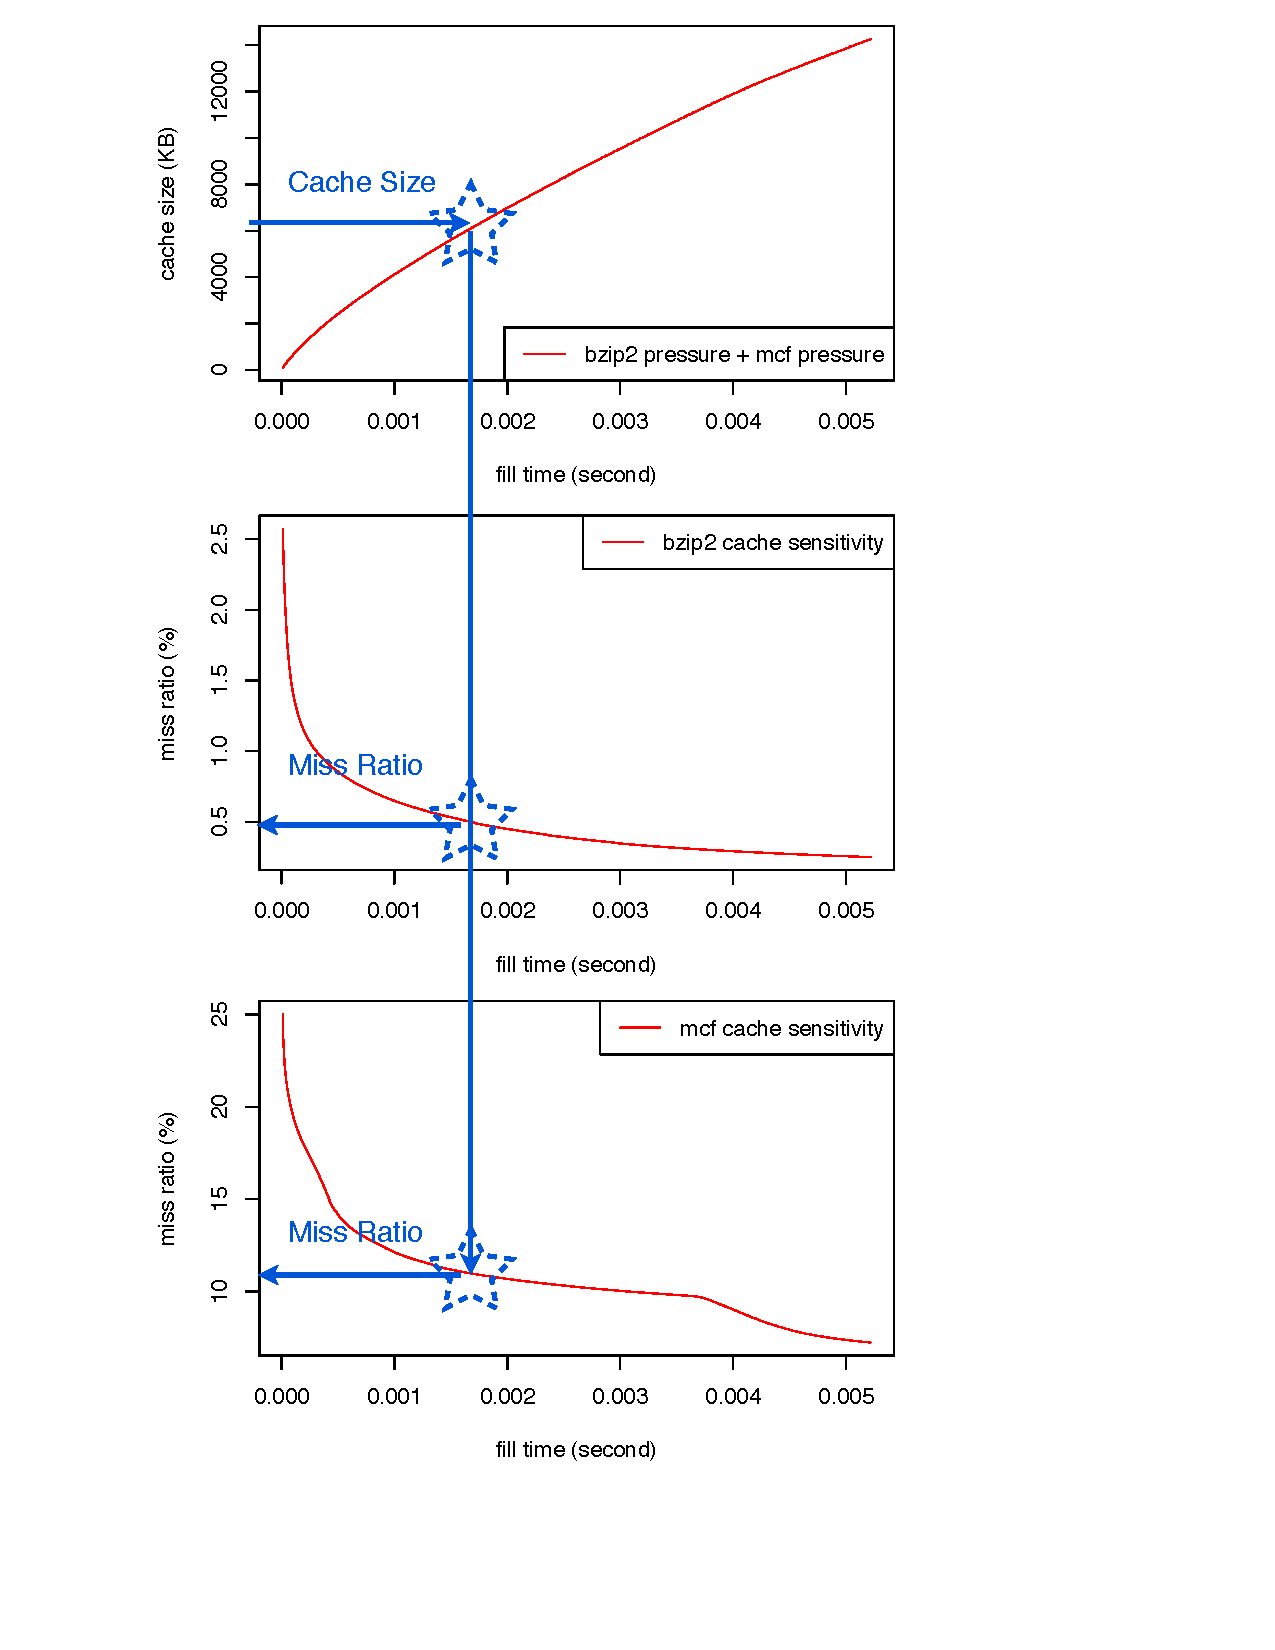
\includegraphics[width=7.5cm,type=pdf,ext=.pdf,read=.pdf]{figures/corun/mix_compute_mr}
\caption{The co-run execution of \emph{bzip2} and \emph{mcf}.  The miss ratios ($M$ for each program) are predicted for the shared cache size $C$.  The combined pressure plot is used to read the fill time on its $x$-axis.  The fill time is used in each of the sensitivity plots to find the shared-cache miss ratio. }
\label{fig:mix_compute_mr}
\end{figure}

As abstractions, these models may not be accurate.  We have discussed
the source of errors due to phase behavior.  The co-run programs may
each have phase behavior.  On the one hand, the number of phase
combinations is much greater.  On the other hand, at least for
independent programs, the phases are not synchronized and may be more
likely to produce the average behavior predicted by the model.

Another complication is the non-uniform effect of cache sharing.  Our
time model assumes that the speed of execution of all programs changes
by the same relative amount.  It has been observed and explained that
co-run slowdown is asymmetrical (e.g.~\cite{Zhang+:EuroSys09}).  The
iterative model we introduced in Section~\ref{sec:iter-model} used an
iterative solution to compute the mutual effect on time dilation until
it converged. The prediction from the new model can be used as the
input to the iterative solution.  In this paper, we maintain the
simplicity and will evaluate the accuracy of the model without this or
other refinements.

By now we have defined the two shared-cache metrics and shown that
they are sufficient, after simplifications mentioned earlier, to predict
the shared-cache performance of any number of co-run programs for any
cache size.

\section{Evaluation}

\subsection{Iterative Model}
\label{sec:iter-rank}
\paragraph{Experimental design}
We apply both all-footprint analysis and average-footprint analysis to
the iterative model to evaluate 1)the accuracy of iterative model and
2)the representativeness of average footprint. To evaluate
cache-sharing predictions, we run two sets of experiments:  

\begin{itemize}
\item 2-program co-runs. We predict all 2-program co-runs and compare
  the predicted ranking with that of the previous work using the 15 SPEC
  2000 benchmarks.

\item 3-program co-runs. We evaluate the prediction for all
  program triples of 8 representative benchmarks in SPEC2006 as
  selected by Zhuravlev et al.~\cite{Zhuravlev+:ASPLOS10}.
\end{itemize}


\paragraph{Two-program co-run ranking}
\label{sec:2-corun}
We run our test set of 15 programs on a dual-core machine that has
2.0GHz Intel Core Duo processor with two cores sharing 2MB L2 cache
and 2GB memory.  There are ${15 \choose 2} = 105$ ways of
pairing two of the 15 programs to share cache. We use all-footprint
analysis and average-footprint analysis on each of 15 programs in a
sequential run and use the iterative model to rank cache interference
of co-run choices.  The ranking is based on the predicted slowdown
(the geometric mean in each group). To show how useful the model is in
predicting the performance of shared cache, we evaluate the ranking by
measuring the change in the actual execution time. To measure the
interference, we run a pair of programs long enough and take the
average slow down, following the method used in~\cite{Zhang+:EuroSys09}. 

We evaluate the prediction by plotting an \emph{interference-ranking
  graph}. The prediction results are shown in a 2-D plot.  The
$x$-axis is the rank of program co-run groups.  In this test, the rank
ranges from 1 (the least interfering pair) to 105 (the most
interfering pair).  The $y$-axis shows the interference, measured by
the quadratic mean of the slowdowns of programs in the co-run group.
The slowdown of a co-run program is the ratio of its co-run time and
the time running alone on the same machine (cache).  For two programs
with slowdowns $s_1,s_2$, we have $y = \sqrt{ \frac{s_1^2 + s_2^2}{2}}$.

\begin{figure}[h!]
\centering
\subfigure{
  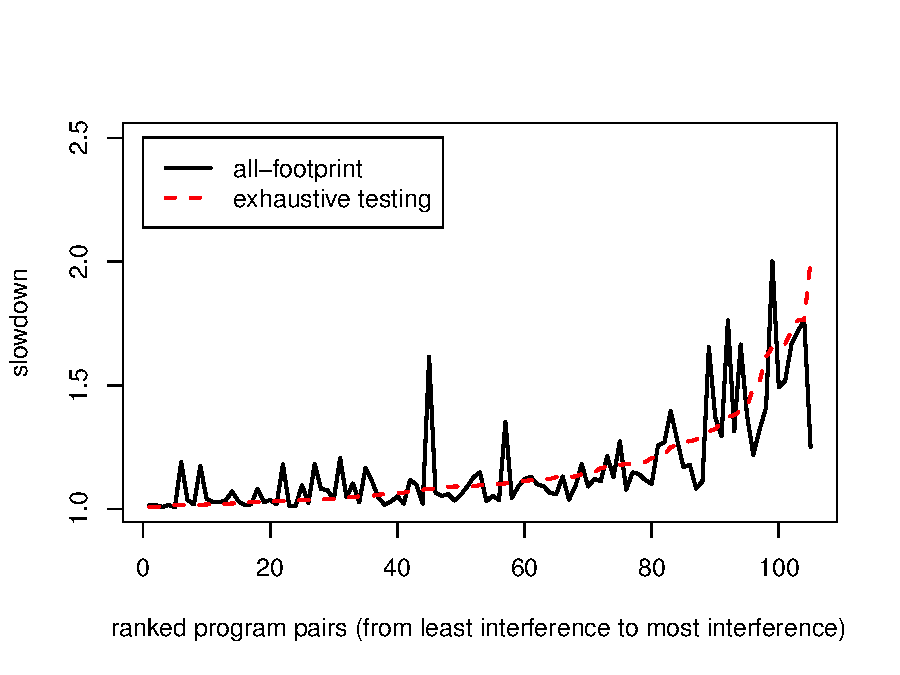
\includegraphics[width=0.6\textwidth]{figures/corun/paw}
}\\
\subfigure{
  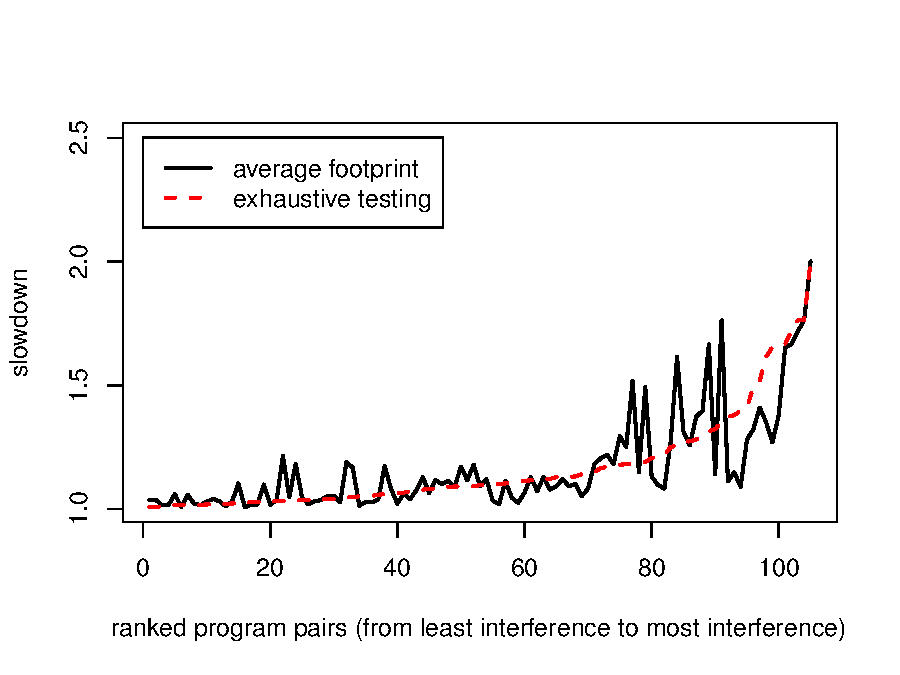
\includegraphics[width=0.6\textwidth]{figures/corun/fix}
}\\
\caption{Evaluation of 2-program co-run predictions for 15 SPEC2000
  benchmark programs.  The prediction quality of average-footprint analysis is similar to that of all-footprint analysis.}
\label{fig:2corun}
\end{figure}

\begin{figure}[h!]
\centering
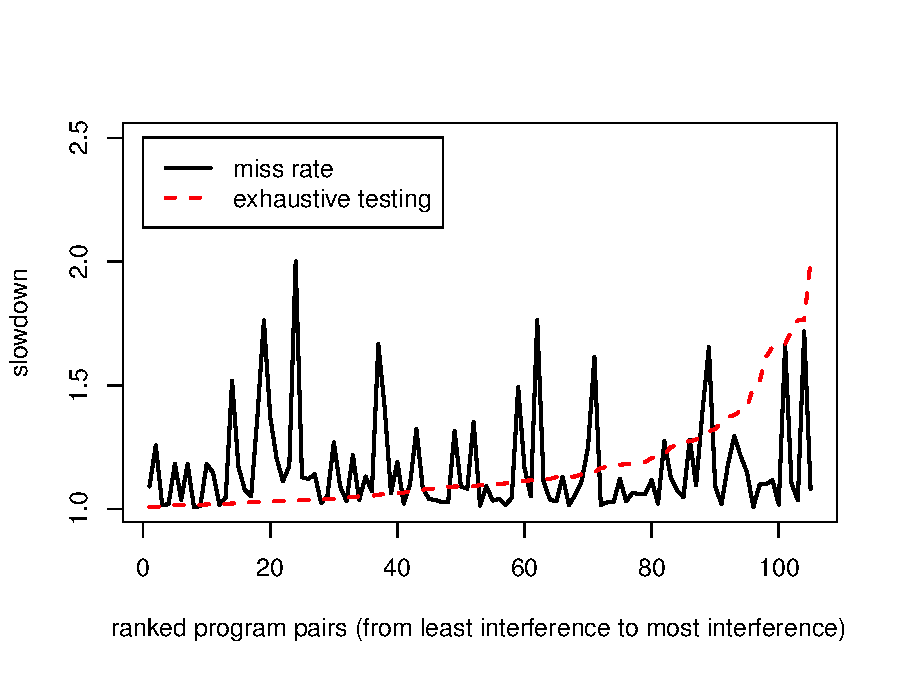
\includegraphics[width=0.6\textwidth]{figures/corun/mr}
\caption{Evaluation of 2-program corun predictions with miss-rate
  based method.}
\label{fig:2corun-mr}
\end{figure}

The three graphs in Figure~\ref{fig:2corun-mr} and
Figure~\ref{fig:2corun} show the plots for the predictions based on
miss rate(by ranking the total miss rate of the programs in the
co-run group), all-footprint analysis, and average-footprint
analysis. In each plot, the accurate result from exhaustive testing is
shown by a monotonically increasing red line as a reference.

The simple miss-rate based prediction does not show an increasing trend,
suggesting no correlation between the prediction and the actual
interference.  The two footprint-based predictions show significant
correlation.  Programs predicted to have a high interference tend to
actually have a high interference.  

Average-footprint analysis ranks several program pairs better than
all-footprint analysis. Consider the pair with the highest
interference, \emph{art,mcf} with a slowdown of 2.  The pair is ranked
23 by miss rate, 99 by all-footprint analysis, and 105 by
average-footprint analysis.  The average-footprint rank is precisely
correct.

All-footprint ranking has a significant misprediction for the program
pair \emph{gcc,art}.  The pair slows down each other by 1.6 times.  It
should be ranked 97 but ranked 44 by all-footprint analysis, which is
worse than the miss-rate rank 70.  The rank by average-footprint
analysis is relatively the best at 86. 

\paragraph{Three-program co-run ranking}

Evaluating larger group co-runs is difficult because the number of
tests increases exponentially with the size of co-run group.  To test all
3-program co-runs in SPEC 2006 benchmarks, we would have to run
${27\choose3} = 2925$ tests.  Even if we ran all the tests, it would
have been impossible to show the results clearly.  Fortunately,
Zhuravlev et al. have analyzed the benchmark set based on the cache
miss rates and access rates and identified 10
representatives~\cite{Zhuravlev+:ASPLOS10}.  We had to narrow
down further because the reuse-distance analysis could finish only for
8 out of the 10 representatives:  $403.gcc$, $416.gamess$, $429.mcf$,
$444.namd$, $445.gobmk$, $450.soplex$, $453.povray$, and
$470.lbm$. There are 56 different 3-program groups from these 8
benchmarks. We show the prediction results in Figure~\ref{fig:3corun}. 

\begin{figure}[h!]
\centering
\subfigure{
  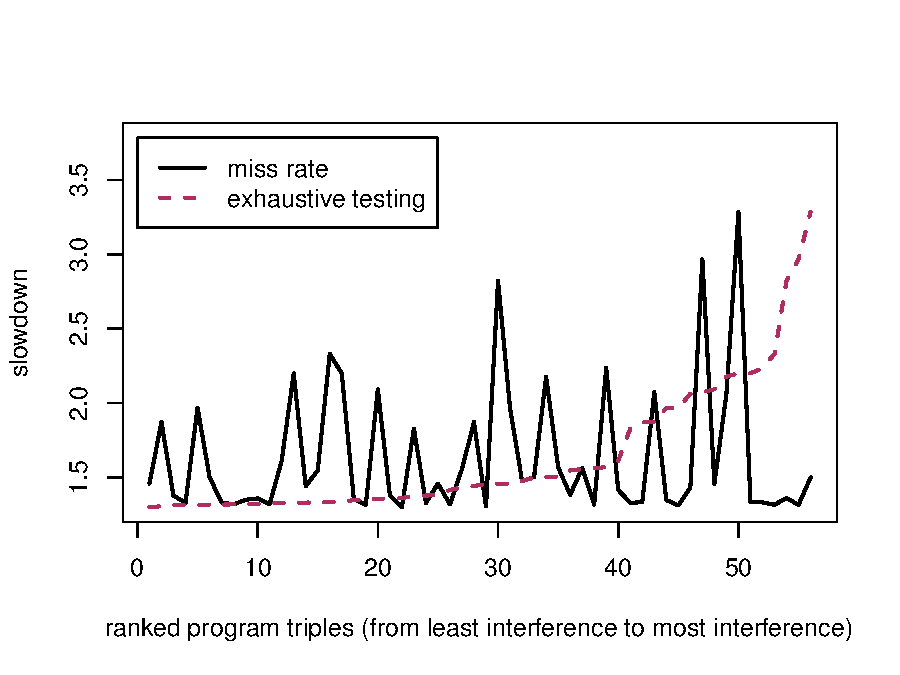
\includegraphics[width=0.6\textwidth]{figures/corun/3mr}
}\\
\subfigure{
  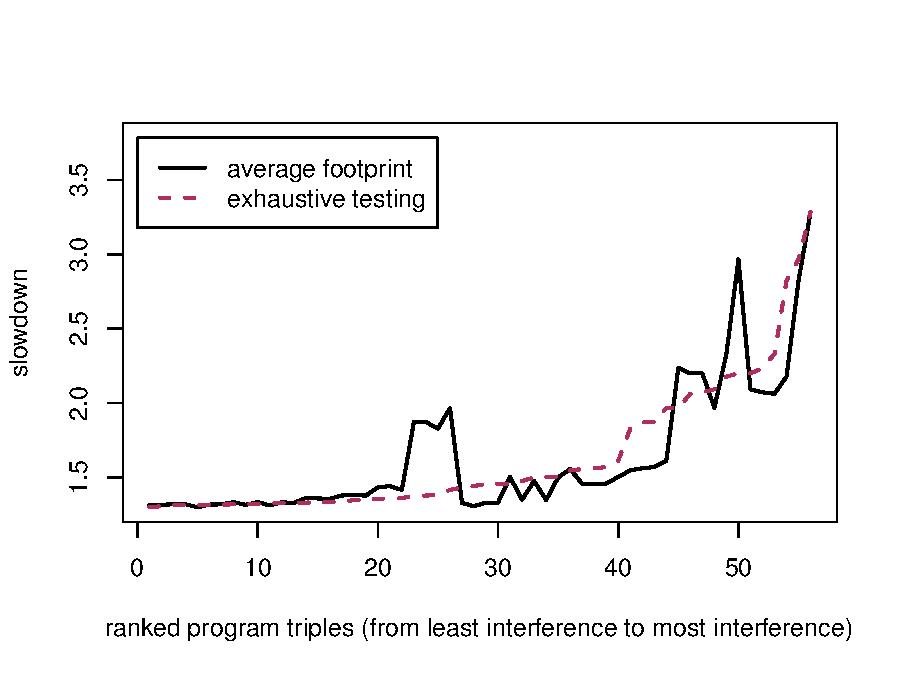
\includegraphics[width=0.6\textwidth]{figures/corun/3rd}
}
\caption{Comparison of 3-program co-run predictions for 8 SPEC2006
  benchmarks.  All-footprint analysis cannot model these programs
  because of its high cost.}
\label{fig:3corun}
\end{figure}

The results for 3-program co-runs of SPEC 2006 programs are similar to
those of 2-program co-runs of SPEC 2000 programs.  As before, the
miss-rate based prediction does not show a detectable correlation
while the average-footprint analysis shows a clear correlation with the
actual interference.

The maximal slowdown increases from 2.0 in 2-program co-runs to 3.3 in
3-program co-runs, confirming the expectation that the interference
becomes worse as the cache is shared by more programs.
Exhaustive testing is also increasingly infeasible.  For both reasons, the
composable model is more valuable, so is the higher efficiency from the
average-footprint analysis.  

\paragraph{Rank and performance closeness}

To quantify the difference between the predicted ranking and the
accurate ranking, we define two metrics: the rank closeness and the
performance closeness.  The \emph{rank closeness} shows on average how
the predicted rank of a co-run group differs from the actual rank.
We number $n$ co-run groups by their accurate rank $i$.  Let $pred(i)$
be the predicted rank for group $i$.  The rank closeness is defined as

$$\text{rank closeness} = \frac{\sum_{i=1}^n | pred(i) - i |}{n}$$ 

\noindent The formula is the Manhattan distance between two vectors
$<p(1), p(2), \dots, p(n)>$ and $<1,2,\dots,n>$, divided by $n$.
The worst possible ranking has a rank-closeness score of $n/2$ if $n$
is even or $(n-1)/2$ otherwise.

% what's the expected closeness from random ranking?

Next we quantify the error in terms of the mis-predicted
slowdown.  Let $f(i)$ be the slowdown of the co-run group with the
accurate rank $i$, and $f(pred(i))$ be the slowdown of the co-run group
with the predicted rank $i$.  The difference $|f(pred(i)) - f(i)|$
gives the mis-prediction. The performance closeness is the average
mis-prediction for all groups:

$$\text{performance closeness} = \frac{\sum_{i=1}^n | f(pred(i)) - f(i)|}{n}$$ 

The two metrics are shown in Table~\ref{tbl:compare-dis}.  On average
for 2-program co-runs, the miss-rate rank errs by 35 positions, while
the footprint-based ranks err by 14 and 15 positions.  For 3-program
co-runs, the miss-rate rank errs by 19 positions, while the
average-footprint rank errs by 6.  In terms of performance, the
miss-rate based ranking mis-predicts twice as bad as the
footprint-based ranking. 

\begin{table}[h]
\centering
\begin{tabular}{|l|c|c|c|}
\multicolumn{3}{c}{2-program co-run over 15 SPEC2000 benchmarks}\\ \hline
ranking strategy       & perf closeness   & rank closeness   \\ \hline \hline
miss rate   & 0.385     & 35       \\ \hline
all-footprint   & 0.194    & 15    \\ \hline
avg-footprint  & 0.170     & 14    \\ \hline
\multicolumn{3}{c}{}\\
\multicolumn{3}{c}{3-program co-run over 10 SPEC2006 benchmarks}\\ \hline
ranking strategy       & perf closeness   & rank closeness  \\ \hline \hline
miss rate   & 0.632     & 19     \\ \hline
avg-footprint  & 0.225     & 6  \\ \hline 

\end{tabular}
\caption{Compare different ranking strategies}
\label{tbl:compare-dis}
\end{table}

In search of a closeness metric, we also measured the Levenshtein
distance.  For two permutations of a set of numbers, the Levenshtein
distance measures the number of ``edits'' needed to convert one to the
other.  For the 2-program co-run test, the distance is 103 for miss
rate, 97 for all-footprint, and 96 for average-footprint.  For the
3-program co-run test, the distance is 54 for miss rate and 48 for
average-footprint. Levenshtein is not a good metric since it does not
distinguish a ranking that does not show a correlation from rankings
that do. 


\paragraph{More results with SPEC2006}
\label{sec:pair}

A complete 2-program co-run test for the 29 SPEC 2006 benchmarks would
include ${29 \choose 2} = 406$ program pairs. We choose 20 programs
out of 29 and reduce the number of pair-run tests to ${20 \choose 2} =
190$. Figure~\ref{fig:co-run} compares the measured and predicted miss
ratios. There are 190 pair runs for a total of 380 executions.  
The $x$-axis orders these executions by the measured miss ratios 
from the lowest to the highest.  For easy viewing, we connect the
points into a line. The measured curve is necessarily monotone.  The
prediction is to match the measurement.

\begin{figure}[t]
  \centering
  %\includegraphics[width=\wid]{../sampling/figures/corun/corun-prediction-20}
  \subfigure[linear scale miss ratios]{
    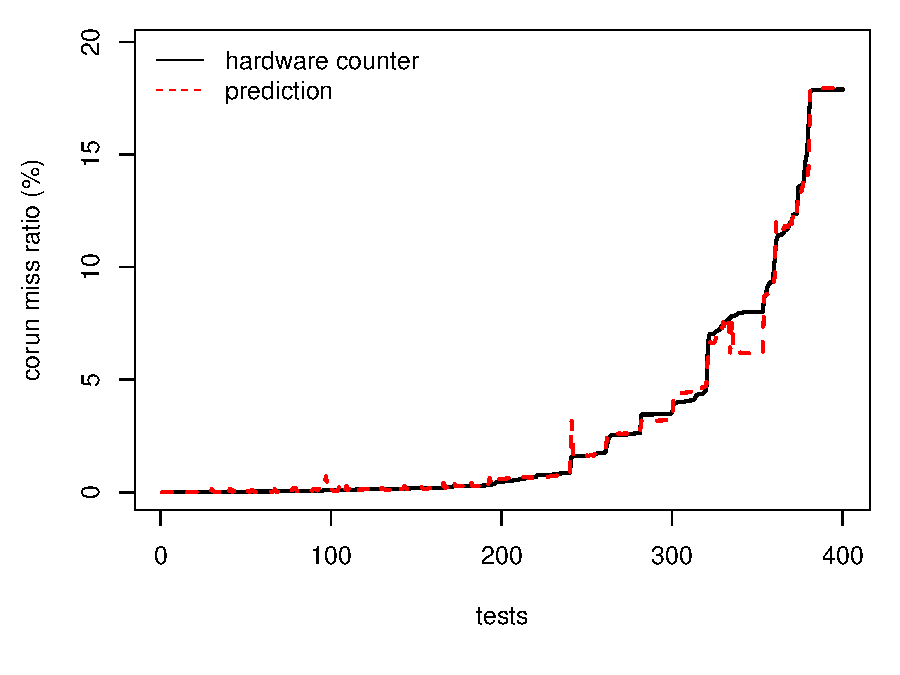
\includegraphics[width=0.4\textwidth,type=pdf,ext=.pdf,read=.pdf]{figures/corun/rank}
  }\hfill
  \subfigure[logarithmic scale miss ratios]{
    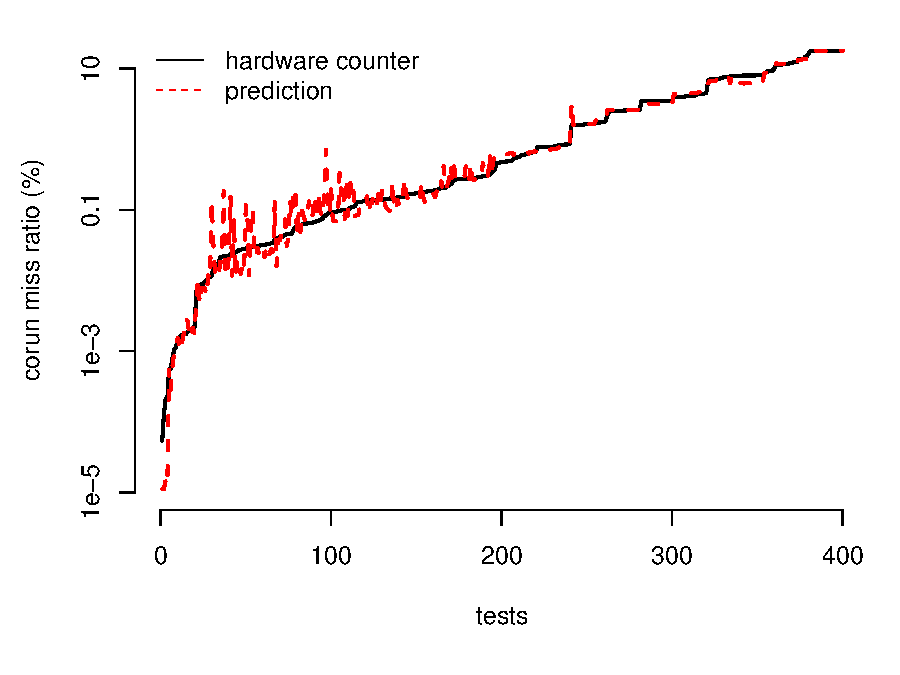
\includegraphics[width=0.4\textwidth,type=pdf,ext=.pdf,read=.pdf]{figures/corun/rank_log}
  }\hfill
  \caption{The predicted and measured miss ratios of the 380
    executions in 190 pair runs. The executions are ordered by the
    ascending miss ratio as measured by the hardware counters in
    exhaustive testing.  For each execution, the solid (black) line
    shows the hardware counter result, and the dotted (red) line shows
    the prediction.  The prediction takes about a \emph{half} percent of the
    time of exhaustive testing.  Just two executions have a significant
    error in both graphs, which are a \emph{half} percent of all executions.}
  \label{fig:co-run}
\end{figure}

Figure~\ref{fig:co-run} has two graphs, showing the miss ratio in the
linear scale in the upper graph and the logarithmic scale in the lower
graph.  The prediction is mostly accurate.  The errors happen but 
for different executions in the two graphs.  If an error is visible in
the linear scale but not in the logarithmic scale, the error is
significant in absolute terms but not in relative terms.  Similarly,
we have errors significant relatively but not absolutely.  The two
graphs show just two errors that are significant in both scales.
% at the index ? and ? (what are the two programs and their pairings?).
In the other 378 (99.5\%) executions, the prediction is either
accurate or the error insignificant.  From visual 
inspection, the error is significant in just 0.5\% of all executions.

To make the prediction, the analysis needs 1 hour 4 minutes CPU time
for sampling, almost as fast as we can run the 20 programs without
analysis.  In comparison, the exhaustive testing takes over 9 days
(estimated) of CPU time.  The cost saving is 99.5\%. 

To see interference in
3-program co-runs, the exhaustive testing has to re-test and collect
results anew, but the modeling needs no additional testing.
Indeed, the new model has been used in an on-line system 
to regroup eight programs to run on two quad-core processors 
(to have a higher performance or at least a more repeatable
performance). We will introduce the system in
Chapter~\ref{chap:regroup}. The exhaustive testing of the 4-program
co-runs in our 20-program suite would need 19 thousand test executions
and have taken months of time. To summarize the pair interference
experiment, we can say that the result is half and half: the modeling
takes half percent of the time and has a significant error in a half
percent of executions. 

\subsection{Pressure-Sensitivity Model}
\paragraph{Experiment design and implementation}
We have tested the full set of 29 SPEC2006 benchmarks and 13 benchmarks
from the PARSEC v2.1 suite. For SPEC 2006, we use the first reference
input provided by the test suite.  The length of SPEC 2006 traces
ranges from 20 billion in \emph{403.gcc} to 2.1 trillion in
\emph{436.cactusADM}.  The amount of data ranges from 3MB in
\emph{416.gamess} to 1.7GB in \emph{429.mcf}.  

We instrument the test programs using Pin~\cite{Pin:PLDI05}, run the
linear-time algorithm to measure the average
footprint(Section~\ref{sec:avg-fp}) and invert it to obtain the fill
time. In the same profiling run with no additional cost, we measure
the reuse-time histogram.  At the end of profiling, we have the cache
pressure and sensitivity. Profiling is done on a Linux cluster where
each node has two Intel Xeon 3.2GHz processors.  The cost is about 38
times slowdown compared to the unmodified execution when profiling the
whole trace (and 0.5\% if we use sampling), as reported in
Table~\ref{tbl:speed}. Our data collection is machine independent.
The measured fill time is the same regardless which hardware
environment is used for data collection.  We will use hardware
counters to verify the modeling results. 

The SPEC suite has 29 programs.  To reduce the cluster in the graphs
we show, we choose a subset of programs.  To avoid bias, we pick
programs with the smallest benchmark ids.  We profile data accesses
only.  This becomes a problem when comparing with the hardware counter
results since the actual miss ratio includes code misses.  For this
reason we removed \emph{perlbench} and \emph{gcc} from the first 22
programs because their code size is large enough to matter to cache
locality.  After the removal, we have 20 SPEC benchmark programs in
our test set, from \emph{401.bzip2} to \emph{464.h264ref}.

For PARSEC, we use the simlarge input.  We run each benchmark with 1, 4,
16, and 64 threads.  Pin can handle multithreaded programs.  We
interleave the memory access traces of the parallel threads and
process the interleaved sequence as a sequential trace.  The parallel
executions are profiled on a machine with two 6-core 2.53GHz Intel
Xeon E5649 processors.

For program co-run testing, we use a machine with two quad-core
2.27GHz Intel Xeon E5520 processors.  The last level (level three)
cache is 4MB per processor, 16-way set associative.  We run two
programs on the same processor.  To measure the actual number of cache
misses, we use Intel's VTune tool to record three hardware counter
events named 

\begin{tabular}{l}
\texttt{OFFCORE\_RESPONSE\_0.DATA\_IN.LOCAL\_DRAM} \\
\texttt{MEM\_INST\_RETIRED.LOADS} \\
\texttt{MEM\_INST\_RETIRED.STORES} \\
\end{tabular}

\noindent The miss ratio is the first count divided by the sum of the
last two counts. 

In modeling, the time is first measured logically by the number of
data accesses.  Then we convert it to real time as follows.  Let
$w_{logical}$ be a time period, e.g. the fill time, measured in the
number of memory accesses, $N$ the total number of memory accesses,
and $T$ the measured solo-run time without instrumentation.  The
corresponding real time $w_{real}$ is

\begin{equation*}
w_{real} = w_{logical} * T / N
\label{eq:time}
\end{equation*}

\begin{comment}
462.libquantum   851.180780780781
437.leslie3d     1151.30810810811
429.mcf  1303.83183183183
433.milc         1431.75495495495
450.soplex       1471.11591591592
410.bwaves       1535.07747747748
459.GemsFDTD     1549.83783783784
434.zeusmp       4575.71171171171
447.dealII       5608.93693693694
436.cactusADM    7695.06786786787

401.bzip2        21963.4162162162
454.calculix     34795.0894894895
456.hmmer        45186.3831831832
458.sjeng        47233.1531531532
445.gobmk        58883.9975975976
435.gromacs      59041.4414414414
464.h264ref      135716.593393393
444.namd         260727.005405405
416.gamess      inf
453.povray      inf
\end{comment}


\paragraph{Pressure and sensitivity of sequential code}

Once we collected the data and sorted the 20 SPEC programs by their fill
time for the 4MB cache, we were surprised to find that they form two
well-separated groups.  Half of the programs have short fill times
from 0.0009 to 0.008 second.  The other half have much longer fill
times from 0.02 to infinity (data size less than 4MB).  If we take the
analogy of pressure as weights, the lightest program in the first
group weighs 2.5 times of the heaviest program in the second group.
We call them high- and low- pressure groups.

It is not the case that floating-point programs have a higher pressure
than integer programs.  Among the 20 programs, two of the three
heaviest, \emph{libquantum,mcf}, are integer programs, and all three
lightest, \emph{namd,gamess,povray}, are floating-point programs,
as can be seen in Figure~\ref{fig:spec06-ps}.

\begin{figure}[t!]
\centering
  \subfigure[The cache pressure of the high-pressure group]{
    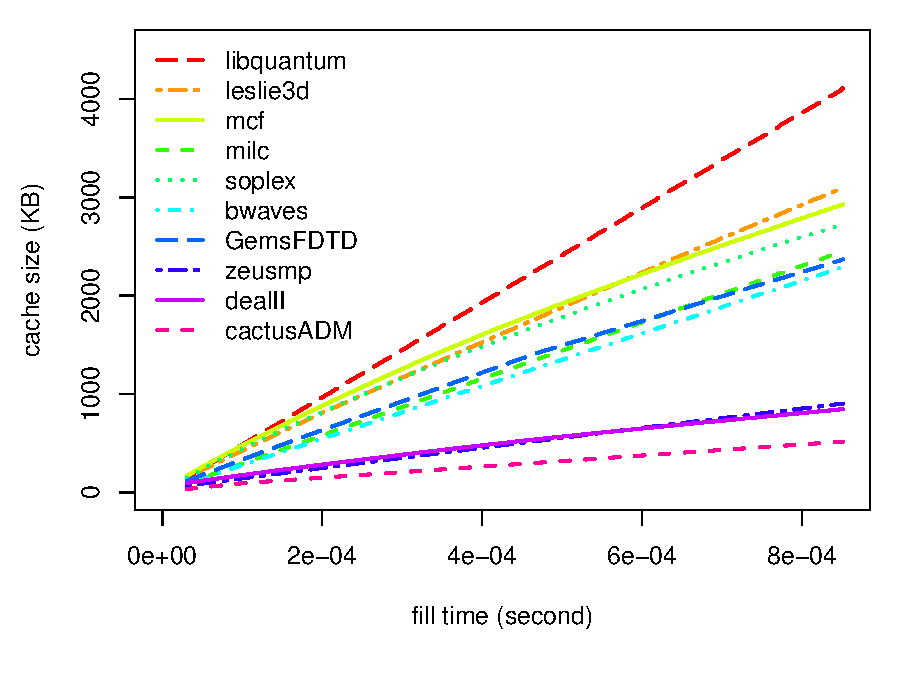
\includegraphics[width=0.47\textwidth,type=pdf,ext=.pdf,read=.pdf]{figures/corun/pres1st}
  }\hfill
  \subfigure[The cache pressure of the low-pressure group]{
    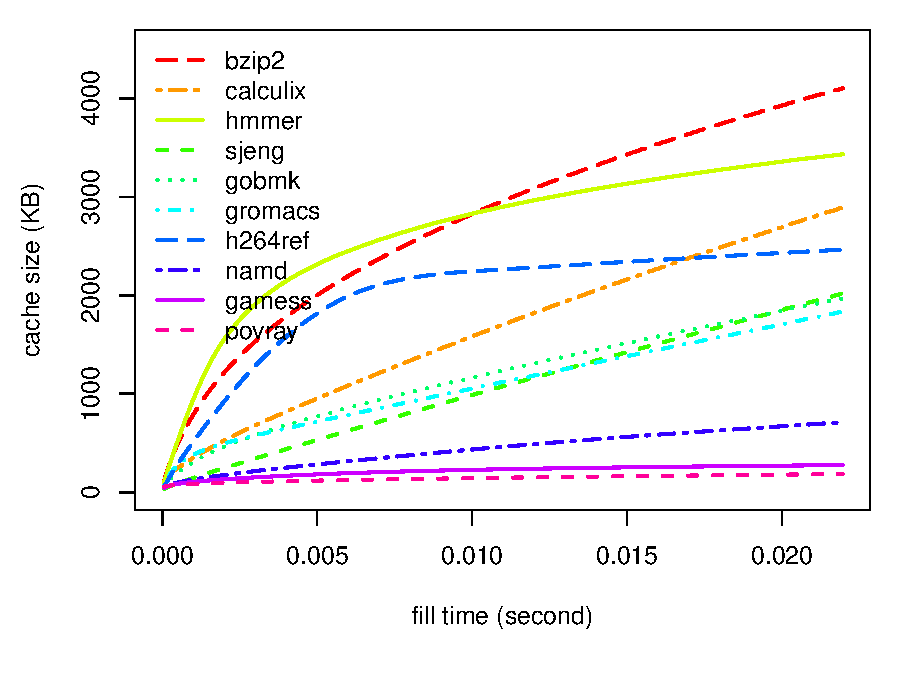
\includegraphics[width=0.47\textwidth,type=pdf,ext=.pdf,read=.pdf]{figures/corun/pres2nd}
 }\hfill
  \subfigure[The cache sensitivity of the high-pressure group]{
    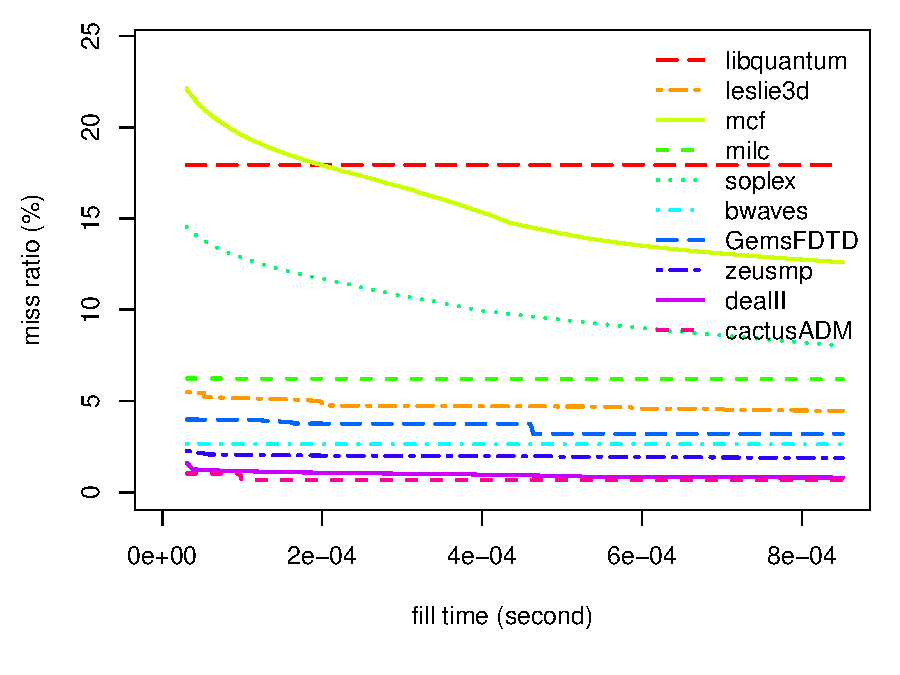
\includegraphics[width=0.47\textwidth,type=pdf,ext=.pdf,read=.pdf]{figures/corun/sens1st}
  }\hfill
  \subfigure[The cache sensitivity of the low-pressure group]{
    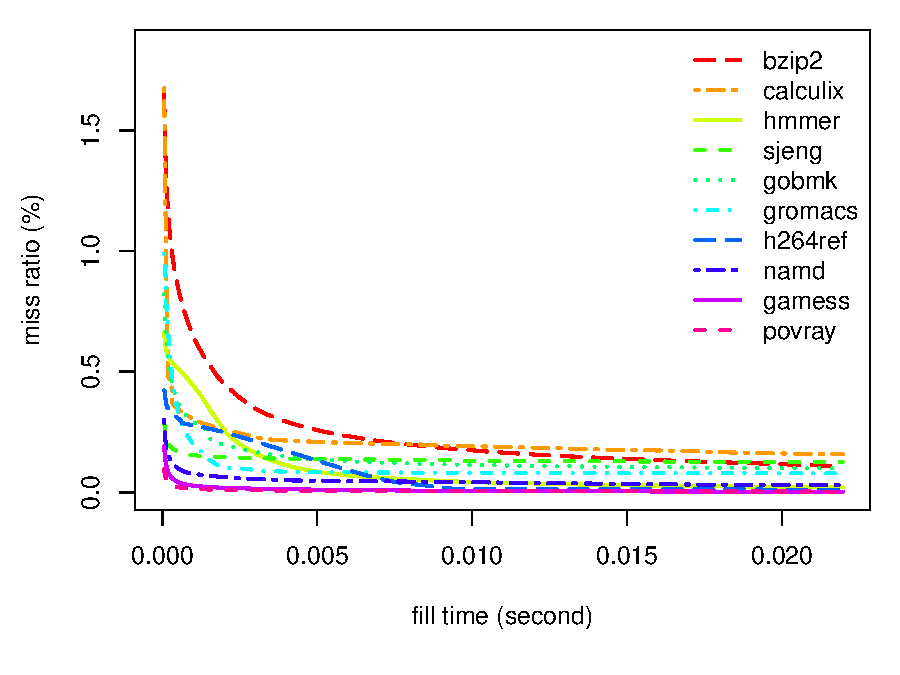
\includegraphics[width=0.47\textwidth,type=pdf,ext=.pdf,read=.pdf]{figures/corun/sens2nd}
 }\hfill
\caption{The cache pressure and sensitivity of 20 SPEC 2006 benchmark programs}
\label{fig:spec06-ps}
\end{figure}

Figure~\ref{fig:spec06-ps} shows 4 graphs plotting the pressure and the
sensitivity for the two groups.  Due to the large difference in
pressure, we use very different fill times on the $x$-axis.  The
high-pressure group fills cache faster, so the plotted range of the
fill time is 1/25 of that of the low-pressure group.

The two pressure graphs show a factor of 10 spread within each group,
showing a wide range in the intensity of the shared cache activity by
the benchmark programs.  Six high-pressure programs and one
low-pressure program have straight lines.  The linear relationship
between the fill time and the cache size means a constant flow rate.
The majority, 13 programs, have some variation.  The greatest is
\emph{h264ref}, with a rapid pressure rise before 2MB and a much
slower climb after 2MB.

The two sensitivity graphs differ by a factor of 13 in the range of
the miss ratios on the $y$-axis.  Most of the heavy weight programs
have much higher miss ratios than the other programs do.  Half of them
show a straight line, the unambiguous mark of insensitivity.  Two of
them and all the light-weight programs have a significant down slope,
which marks the sensitive area where the miss ratio may change sharply
depending on the co-run environment.  

\paragraph{Program personality in shared cache}

To compare programs directly, we fix the cache size so each program
has a single number for the pressure and for the sensitivity.  Visually,
this is done using the graphs in Figure~\ref{fig:spec06-ps} as follows.
On the pressure graph, we find the cache size on the $y$-axis, and then
find the fill time on the $x$-axis.  The pressure is the reciprocal of 
the fill time, i.e. the fill rate.  On the sensitivity graph, we find
the miss ratio corresponding to the fill time.  

We plot these two numbers as 2D coordinates with the miss ratio on the
$y$-axis and fill rate on the $x$-axis.  Since the plot includes both
aspects of cache sharing, we call it the \emph{program personality}
chart.  The position in the personality chart completely represents
the interactivity of a program in shared cache.

\begin{figure}[t!]
\centering
  \subfigure[The sensitivity-pressure (program personality) graph, 4MB cache]{
    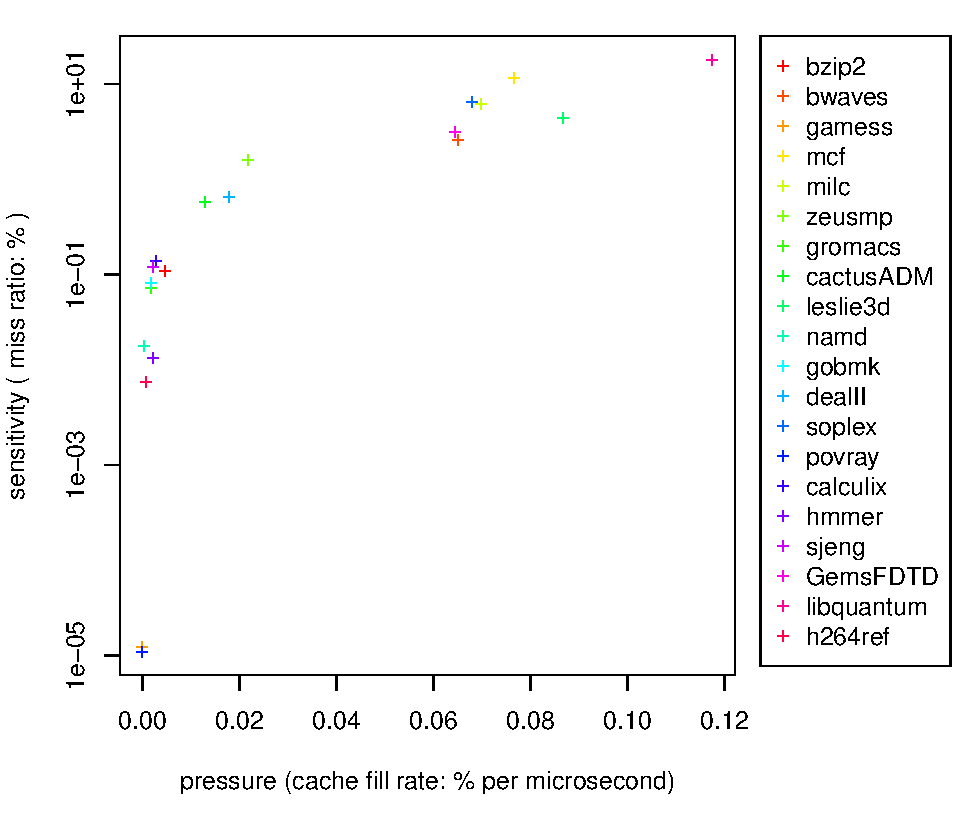
\includegraphics[width=8.5cm,type=pdf,ext=.pdf,read=.pdf]{figures/corun/dist_4m}
  }\hfill
  \subfigure[The sensitivity-pressure (program personality) graph, 32KB cache]{
    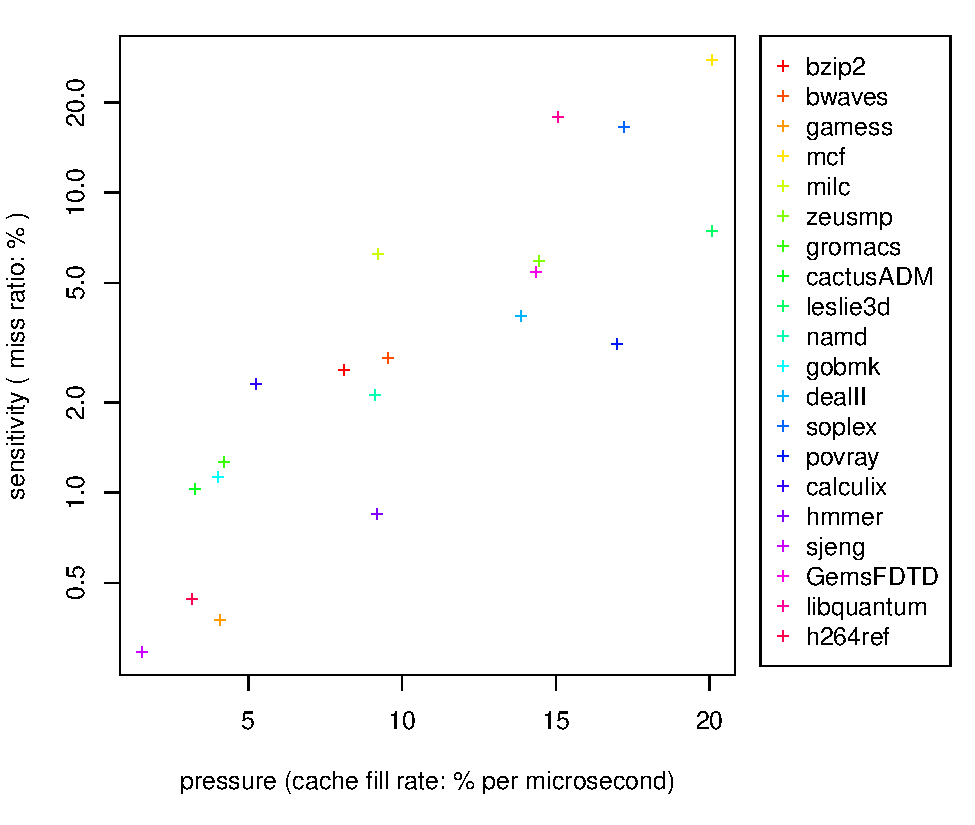
\includegraphics[width=8.5cm,type=pdf,ext=.pdf,read=.pdf]{figures/corun/dist_32k}
 }
\caption{The program personality in shared cache, represented by plotting
  the sensitivity (miss ratio) and pressure (fill rate) in a single
  chart first for the 4MB cache and then for the 32KB cache}
\label{fig:personality}
\end{figure}

Figure~\ref{fig:personality} shows the program personality charts for
the 4MB and the 32KB cache respectively.  The range of personalities
differs in the two cache sizes but the general trend is a band
stretching from the lower-left corner to the upper-right corner.  The
personalities vary from low-pressure and low sensitivity to
high-pressure and high-sensitivity.  Next we show the co-run
interference for the 4 of the 20 programs to cover all the extreme
personalities in shared cache.

\paragraph{Co-run interference}

Prominent in Figure~\ref{fig:spec06-ps}(a,c) the pressure and sensitivity
graphs, \emph{libquantum} is predicted to have the greatest pressure
and zero sensitivity.  We verify this by testing it in 20 co-runs each
with one of the 20 programs (including itself).  We measure its
shared-cache miss ratio using the hardware counters.  The 20 co-run
miss ratios are shown by the 20 bars in Figure~\ref{fig:corun-bar}(a).
They change between 17.82\% and 17.89\%.  Effectively they do not
change, which is the prediction (of around 17.9\%), shown by the 20 bars shown
side-by-side with the measured bars in the same figure.  The
prediction is the direct consequence of the sensitivity curve.  In
fact, the 17.9\% prediction can be read directly from
Figure~\ref{fig:spec06-ps}(c).

The reason for the slight over-prediction (0.1\%) is possibly the
simplifications we made in modeling.  But it is also possibly that the
Intel cache is not strictly LRU while our model assumes (fully
associative) LRU.

\begin{figure}[h!]
\centering
\footnotesize
\subfigure[Co-run interference of \emph{libquantum}; high pressure, zero sensitivity; measured miss ratio 17.82\% to 17.89\%, predicted 17.9437\% to 17.9447\%]{
    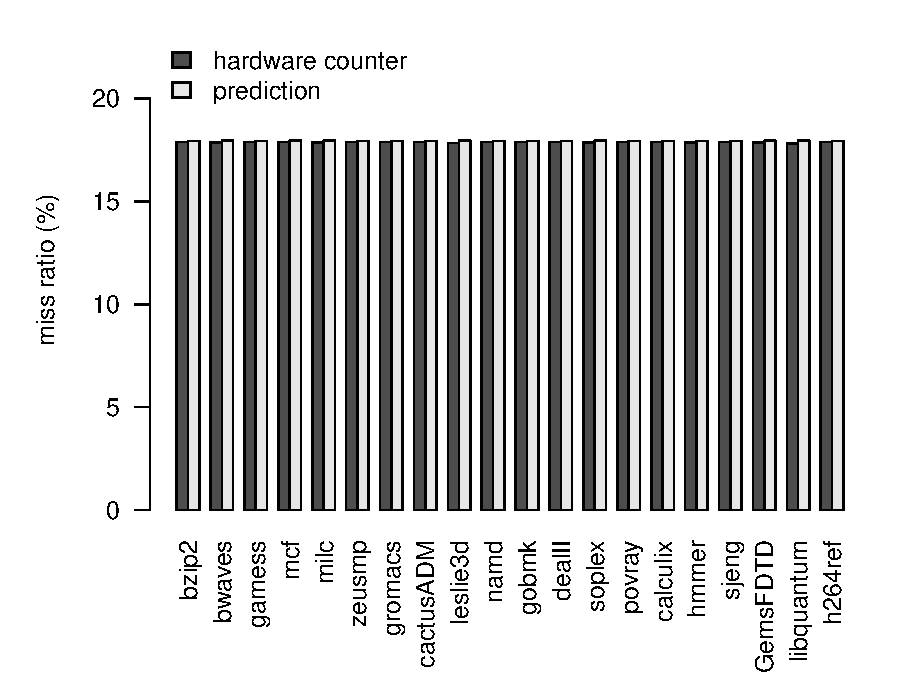
\includegraphics[width=0.47\textwidth,type=pdf,ext=.pdf,read=.pdf]{figures/corun/corun_mr_comp_462.libquantum}
  }\hfill
  \subfigure[Co-run interference of \emph{mcf}; high pressure, highly sensitive; measured miss ratio 11.2\% to 16.4\%, predicted 11.6\% to 14.4\%]{
    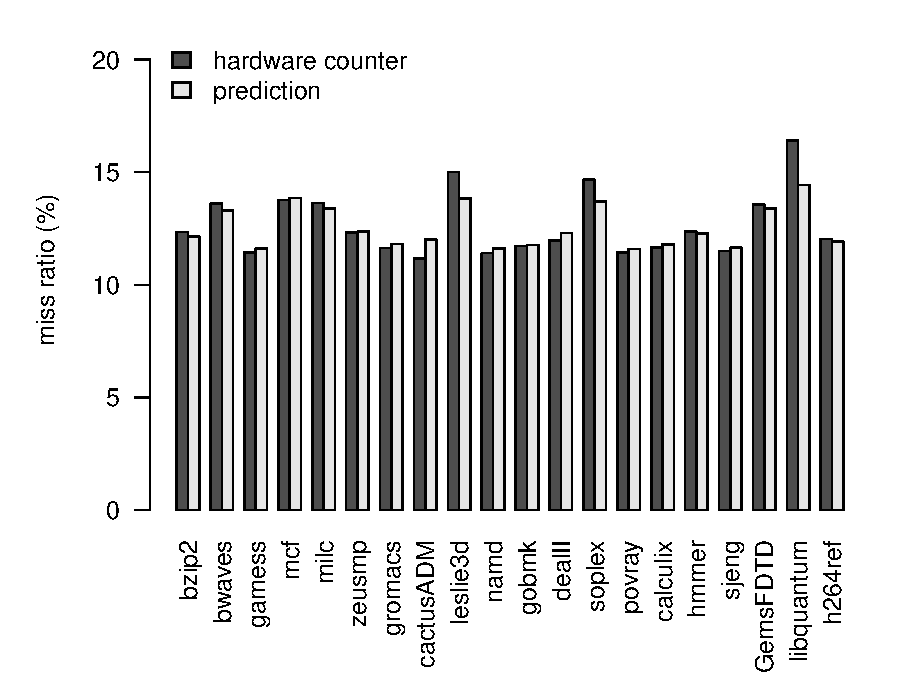
\includegraphics[width=0.47\textwidth,type=pdf,ext=.pdf,read=.pdf]{figures/corun/corun_mr_comp_429.mcf}
  }\hfill
  \subfigure[Co-run interference of \emph{gobmk}; low pressure, highly sensitive; measured miss ratio 0.13\% to 0.33\%, predicted 0.08\% to 0.32\%]{
    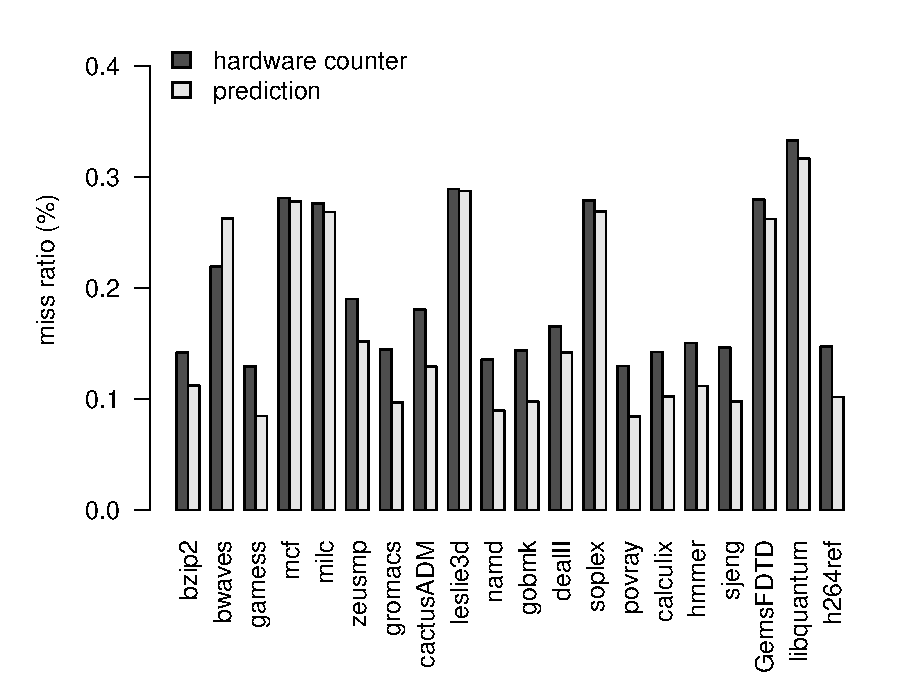
\includegraphics[width=0.47\textwidth,type=pdf,ext=.pdf,read=.pdf]{figures/corun/corun_mr_comp_445.gobmk}
  }
 \hfill
  \subfigure[Co-run interference of \emph{gamess}; low pressure, low sensitivity; measured miss ratio 0.0002\% to 0.04\%, predicted 0.000013\% to 0.03\%]{
    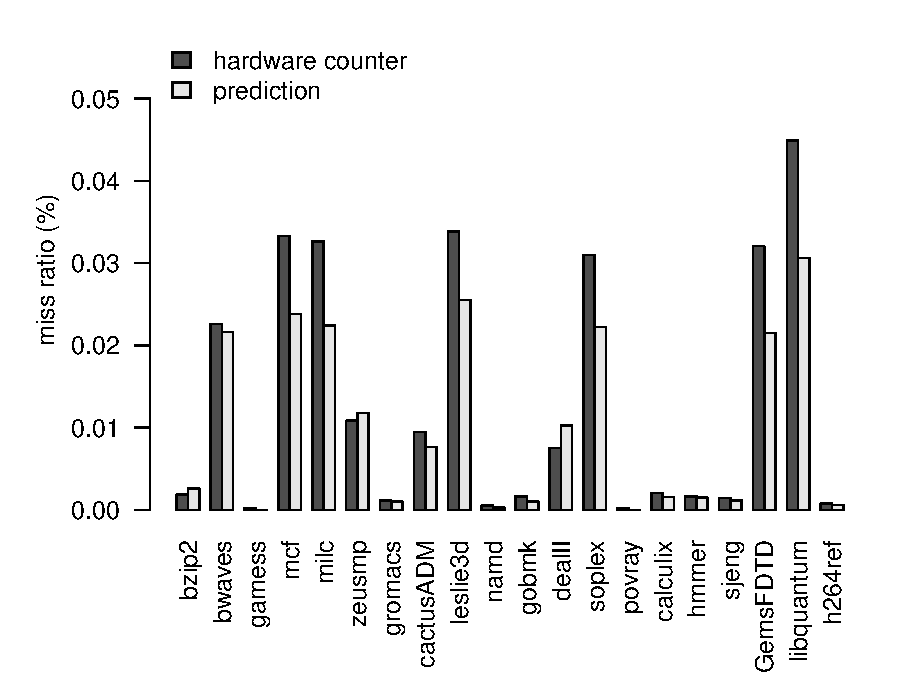
\includegraphics[width=0.47\textwidth,type=pdf,ext=.pdf,read=.pdf]{figures/corun/corun_mr_comp_416.gamess}
  }
  \caption{The predicted and measured co-run miss ratios of four
    programs, each is tested when running with one of the 20 programs
    including itself. The four programs are selected by their
    different shared-cache personality (Figure~\ref{fig:personality}).
    {\bf Note that the measured miss ratios (the $y$-axis in
      these plots) vary by three orders of magnitude.  It is
      remarkable that the software prediction (with no parallel
      testing nor any hardware counter input) matches with the
      hardware measurement in every case.}}
\label{fig:corun-bar}
\end{figure}

\emph{Mcf} is predicted to have a high pressure and high sensitivity.
The measured results in Figure~\ref{fig:corun-bar}(b) confirms this
prediction.  Depending on cache sharing, the actual miss ratio varies
by 5.2\% from 11.2\% to 16.4\%.  The predicted variation is 2.8\% from
11.6\% to 14.4\%.  Among the 20 programs, \emph{Mcf} has one of the
largest performance variations due to cache sharing.

According to the prediction, the next two programs,
\emph{gobmk,gamess}, should have a low pressure.  In addition,
\emph{gobmk} should be highly sensitive, while \emph{gamess} should be
the opposite and highly insensitive.  At the first glance, the
measurement shown by the two graphs in Figure~\ref{fig:corun-bar}(c,d)
does not seem to support the prediction.  If anything, the relative
variation of the insensitive \emph{gamess} is more dramatic.  However,
if we consider the miss ratio numbers, \emph{gamess} is at most
0.04\%, effectively zero.  If Figure~\ref{fig:corun-bar}(d) were plotted
with the same $y$-axis as Figure~\ref{fig:corun-bar}(c), there will be
little visible variation.

The four programs shown here have very different miss ratios, from
$10^{-7}$ to 19\%.  Given the \emph{six} orders of magnitude
difference, just predicting the miss ratio to within the range of the
actual miss ratios would be a commendable result.  The fact our
predictions match the variation in extremely large and extremely small
miss ratios is more than remarkable.  It gives us the greatest
confidence that the new models are not just simple and easy to
understand and use but actually capture the program characteristics
essential to its performance in shared cache.

\paragraph{Parallel code}

Like co-run sequential code, a parallel program has to contend with
the same problem that using more CPU cores leads to higher contention
in the shared cache.  A difference is that parallel threads share
data, so the increase in cache pressure may be moderated.  An
important optimization is to maximize the data sharing.  The new
metrics of pressure and sensitivity may assist such optimization.  In
this section, we show their use in understanding parallel performance.

We have tested the full set of the 13 multi-threaded PARSEC
benchmarks, with 1, 4, 16, and 64 threads.  For space limitation we
choose two programs, {\em dedup, facesim}.  {\em Dedup} compresses a
data stream using both global and local compression through
'deduplication'. The compression kernel exploits pipelined parallelism
and mimics ``real-world implementations.'' {\em Facesim} computes a
visually realistic animation of a human face by simulating the
underlying physics.

We choose these two based on their parallel execution times, shown in
Table~\ref{tbl:parsec_runtime}.  When the number of threads is increased
from 16 to 64, {\em facesim} shows a similar speed but {\em dedup}
loses 83\% performance.  The pair makes a good contrast and case study
in shared cache performance analysis.

\begin{table}[h!]
\centering
\begin{tabular}{|c|c|c|c|c|}
\hline
num. threads & 1 & 4 & 16 & 64 \\ \hline \hline
{\em facesim} & 14.054 & 8.140 & 5.807 & 5.880 \\ \hline
{\em dedup} & 8.267 & 2.817 & 2.930 & 5.276 \\ \hline
\end{tabular}
\caption{{\em Facesim, dedup} exhibit a drastically different effect on
  running time when the number of threads is increased from 16 to 64}
\label{tbl:parsec_runtime}
\end{table}

Figure~\ref{fig:parsec} shows how the pressure and the sensitivity
changes with the number of threads in both programs.  When the number
of threads is increased from 16 to 64, we see a much larger increase
in the cache pressure of {\em dedup} than in {\em facesim} and in the
cache sensitivity of {\em dedup}.  The sensitivity of {\em facesim}
stays virtually the same.  The combination of intensified pressure and 
heightened sensitivity in {\em dedup} should lead to a significant
increase in the miss count, which would explain the 83\% performance
drop.

\begin{figure}[t!]
\centering
  \subfigure[The pressure graph for PARSEC/dedup]{
    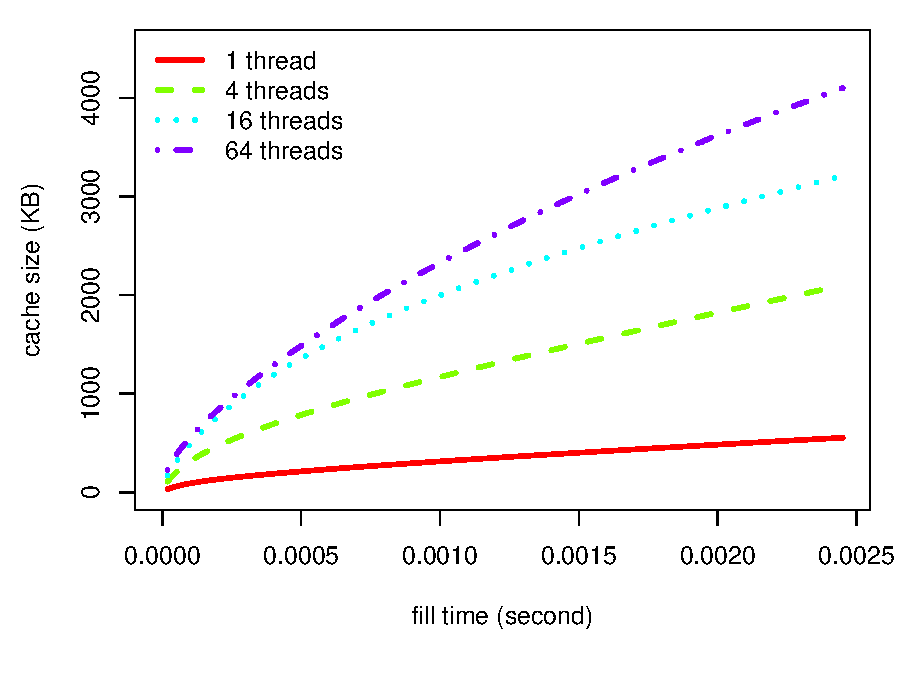
\includegraphics[width=0.47\textwidth,type=pdf,ext=.pdf,read=.pdf]{figures/corun/pres_dedup}
    \label{fig:dedup_pres}
  }\hfill
  \subfigure[The pressure graph for PARSEC/facesim]{
    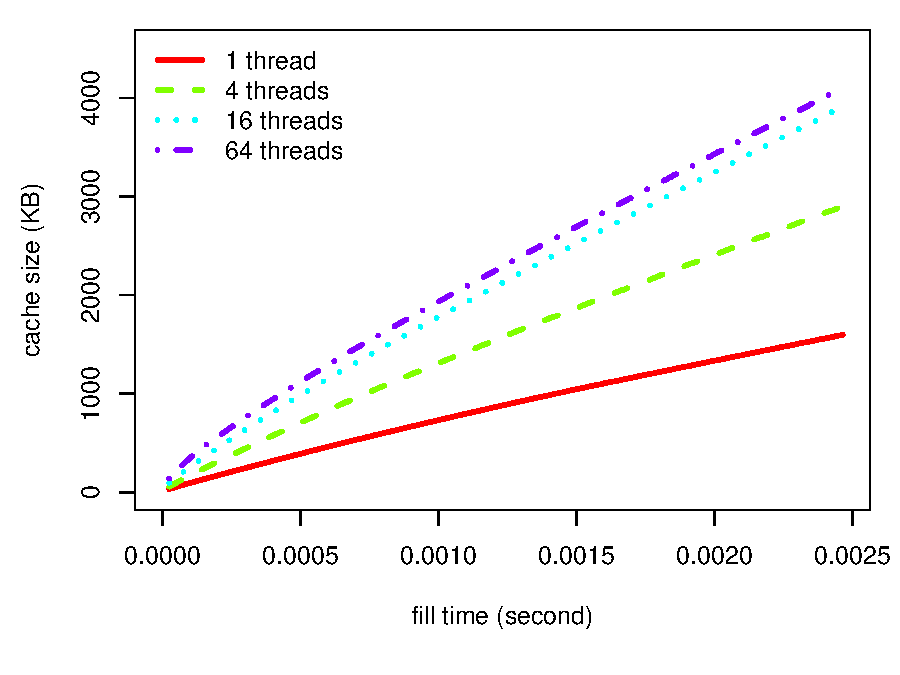
\includegraphics[width=0.47\textwidth,type=pdf,ext=.pdf,read=.pdf]{figures/corun/pres_facesim}
 }\hfill
  \subfigure[The sensitivity graph for PARSEC/dedup]{
    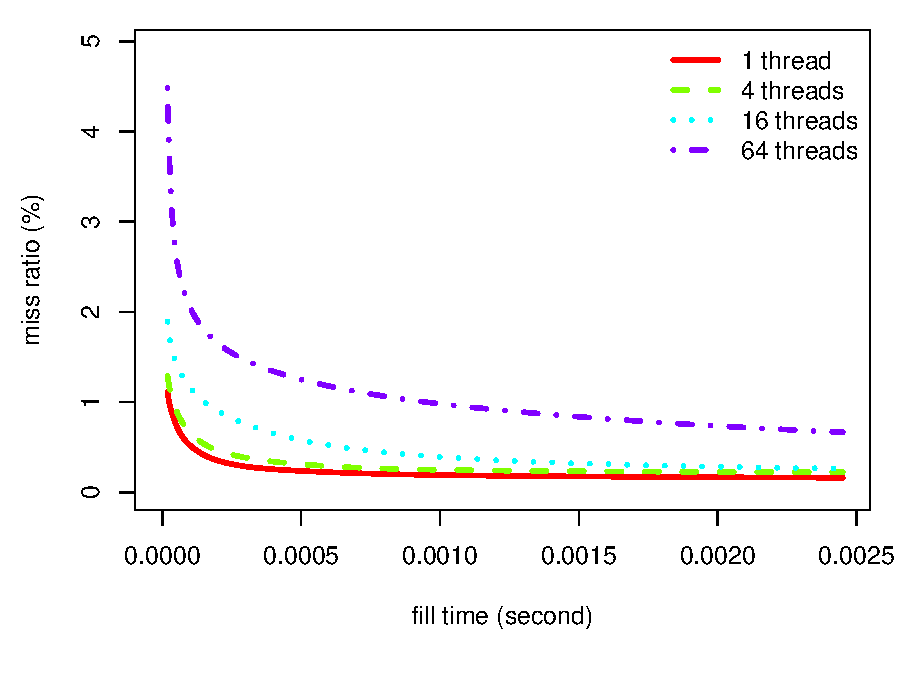
\includegraphics[width=0.47\textwidth,type=pdf,ext=.pdf,read=.pdf]{figures/corun/sens_dedup}
    \label{fig:dedup_sens}
  }\hfill
  \subfigure[The sensitivity graph for PARSEC/facesim]{
    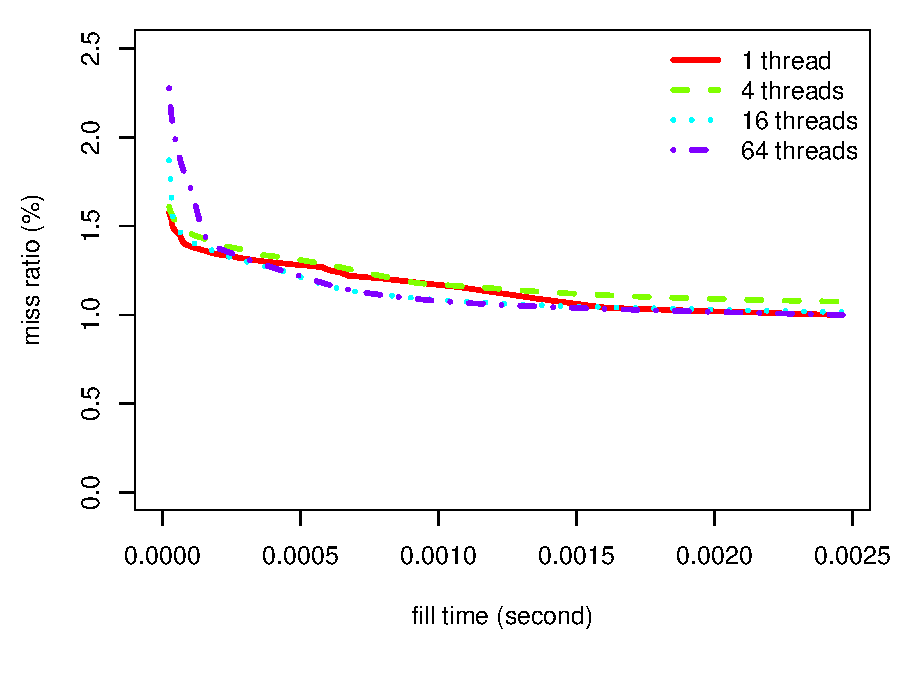
\includegraphics[width=0.47\textwidth,type=pdf,ext=.pdf,read=.pdf]{figures/corun/sens_facesim}
 }\hfill
\caption{The cache pressure and sensitivity of 2 multi-threaded
  programs, running with 1, 4, 16, and 64 threads.  The increase in
  the {\em dedup} pressure and sensitivity at the 64-thread run helps
  to explain the 83\% performance loss shown in Table~\ref{tbl:parsec_runtime}}
\label{fig:parsec}
\end{figure}

Under the other thread counts, the sensitivity of both
programs do not change much.  The parallel execution is not
significantly affected by cache sharing.  Interestingly, {\em Facesim}
becomes less sensitive when adding threads from 4 to 16.  It would be
interesting to investigate what program organization produces this
beneficial effect to improve cache sharing.

\section{Discussion}

We have present two new cache sharing models in this
Chapter. Iterative models focus on programs' circular effect in shared
cache and defines program actions. Pressure and sensitivity models
focus on programs' intrinsic characteristics and defines program
personalities. These two kinds of models can be used either in
different way to explore their best potential or combined together to
aggregate their strength. We will leave it as an topic of future
work. 
